\documentclass[a4paper,11pt,oneside]{report}

% --------------------------------------
% BASIC PACKAGES
% --------------------------------------
\usepackage[utf8]{inputenc}
\usepackage[T1]{fontenc}
\usepackage{fouriernc}
\usepackage{geometry}
\usepackage{setspace}
\usepackage{amsmath, amssymb}
\usepackage{graphicx}
\usepackage{float}
\usepackage{caption}
\usepackage{subcaption}
\usepackage{booktabs}
\usepackage{array}
\usepackage{multirow}
\usepackage{longtable}
\usepackage{enumitem}
\usepackage{xcolor}
\usepackage{listings}
\usepackage{url}

% --------------------------------------
% TIKZ & GRAPHICS
% --------------------------------------
\usepackage{tikz}
\usetikzlibrary{positioning, arrows.meta, shadows, shapes, arrows, fit}
\usepackage{pgfplots}
\usepackage{pgfgantt}
\usepackage{msc}

% --------------------------------------
% CAPTION SETTINGS
% --------------------------------------
\captionsetup{font=small}

% --------------------------------------
% HYPERLINKS & REFERENCES
% --------------------------------------
\usepackage{hyperref}
\usepackage[nottoc]{tocbibind}
\usepackage{csquotes}
\usepackage{cite}  % Numeric citation style

% --------------------------------------
% PAGE GEOMETRY & SPACING
% --------------------------------------
\geometry{margin=1in}
\setstretch{1.3}

% --------------------------------------
% CUSTOM COMMANDS
% --------------------------------------
\newcommand{\plogo}{\fbox{$\mathcal{PL}$}}


\begin{document}

	\begin{titlepage}

		\centering

		\vspace*{\baselineskip}

		\vspace{0.75\baselineskip}

		{\LARGE  EcoSenseNet - Smart Environment Prediction and  Alert System}

		\vspace{0.75\baselineskip}

		\vspace{2\baselineskip}

		A report submitted for the course named Project-III (CS4203)

		\vspace*{7\baselineskip}

		Submitted By

		\vspace{0.5\baselineskip}

		{\scshape\Large Pratiksha\\ SEMESTER - 7TH \\ 220101098}

		\vspace{0.5\baselineskip}

		Supervised By

		\vspace{0.5\baselineskip}

		{\scshape\Large Dr. Sanasam Chanu Inunganbi}

		\vspace{0.5\baselineskip}

		\vfill

		\begin{center}
			
\includegraphics[width=5cm]{report_file/iiit manipur.png}
		\end{center}

	{\scshape\small Department of Computer Science and Engineering\\ Indian Institute of Information Technology Senapati, Manipur \\ October, 2025}

\end{titlepage}

%----------------------------------------------------------------------------------------

\begin{center}
   { \LARGE \textbf{Declaration}}
\end{center}
In this submission, I have expressed my idea in my own words, and I have adequately cited and referenced any ideas or words that were taken from another source. I also declare that I adhere to all principles of academic honesty and integrity and that I have not misrepresented or falsified any ideas, data, facts, or sources in this submission. If any violation of the above is made, I understand that the institute may take disciplinary action. Such a violation may also engender disciplinary action from the sources which were not properly cited or permission not taken when needed.

\vspace{1cm}\hspace{8.5cm} Pratiksha \\
\vspace{1cm}\hspace{9cm} 220101098 \\
\vspace{1cm} DATE: 30-10-2025

\newpage

\begin{center}
	\thispagestyle{empty}

		\begin{table}
			\centering
			
\includegraphics[scale=0.2]{report_file/iiit manipur.png}
			\begin{tabular}{l}
				Department of Computer Science Engineering \\
				Indian Institute of Information Technology Senapati, Manipur \\
			\end{tabular}
		\end{table}
		\par\noindent\rule{\textwidth}{0.4pt}
			Dr. Sanasam Chanu Inunganbi
			\hspace*{\fill} Email: \href{mailto:inunganbi@iiitmanipur.ac.in}{inunganbi@iiitmanipur.ac.in}\\
			Assistant Professor, CSE
			\hspace*{0pt}\hfill Contact No: +91 70058 44201\\[2cm]
			{\Huge \textbf{\emph{To Whom It May Concern}}}\\[2cm]
			\linespread{1.13}
			\large{This is to certify that the project report
                entitled \textbf{" EcoSenseNet - Smart Environment Prediction and  Alert System",} submitted to the department of Computer Science and Engineering, Indian Institute of Information Technology Senapati, Manipur in partial fullfillment for the award of degree of Bachelor of Technology in Computer Science and Engineering is record bonafide work carried out by \textbf{Pratiksha} bearing roll number \textbf{220101098}.}\\[2.0cm]
			\hspace*{2.1in}\large{Signature of Faculty Advisor}\\
			\hspace*{2in}\textbf{(Dr. Sanasam Chanu Inunganbi)}

	\end{center}
        \vspace{0.5cm}
	Signature of the Examiner 1 ............................\\\\
	Signature of the Examiner 2 ............................\\\\
	Signature of the Examiner 3 ............................\\\\
	Signature of the Examiner 4 ............................\\\\

\begin{abstract}
The \textbf{EcoSenseNet - Smart Environment Prediction and  Alert System} presents the design and development of a smart mini-satellite system intended for environmental monitoring and offline communication within a college campus network. The concept comes from frequent network disruptions in Manipur, where internet outages during disasters hinder effective communication and environmental awareness. This project aims to overcome such challenges by creating a localized, self-sufficient network that can predict environmental changes and broadcast alerts completely offline.

The system operates through a multi-phase implementation distributed across three laptops acting as interconnected nodes. In the first phase, Laptop A, located in the administrative block, collects real-time data using sensors such as MQ4, MQ7, MQ135, MQ2, DHT22, and a flame sensor connected to a Heltec LoRa V3 (ESP32). The Arduino IDE is used to log this data into a CSV file at three-minute intervals. Once sufficient readings are captured, the system converts the data into a JSON payload and forwards it to a FastAPI server running locally. The FastAPI backend hosts a pre-trained Long Short-Term Memory (LSTM) model that analyzes recent patterns and predicts environmental conditions—such as gas concentration, temperature, and humidity—for the next three hours.

In the second phase, the prediction results are exported to a locally hosted Reticulum MeshChat web application. Reticulum, operating through the Heltec LoRa transceiver, transmits the forecast data to another laptop (Laptop B) located in the hostel block. This second node receives the message offline via LoRa and rebroadcasts it over a shared Wi-Fi network using Reticulum’s local web relay feature. Students’ laptops (Laptop C) connected to the same Wi-Fi can instantly access the alerts through Reticulum running on specific ports—port 8000 for full message interaction and port 8080 for read-only access.

The system not only transmits automated environmental alerts but also includes an integrated chat interface that allows administrative staff to send important messages to students, ensuring campus-wide communication even during network failures. All these processes operate entirely offline without depending on cloud services or the internet.

By combining IoT-based sensing, machine learning prediction, and decentralized mesh communication, \textbf{EcoSenseNet - Smart Environment Prediction and  Alert System} demonstrates a feasible, low-cost, and resilient environmental monitoring framework. Its hybrid design—merging electronics, embedded systems, and intelligent networking—illustrates how modern technologies can be adapted to create disaster-ready communication systems in rural and educational environments where connectivity is limited.
\end{abstract}




\pagebreak


\begin{center}
{\LARGE \textbf{Acknowledgement}}
\end{center}

I would like to express my deep gratitude to all the individuals and institutions who have supported me throughout the course of this project.\\

First and foremost, I extend my heartfelt thanks to my supervisor, \textbf{Dr. Sanasam Chanu Inunganbi}, for her invaluable guidance, insightful feedback, and unwavering support throughout the development of this project. Her expertise and encouragement have been instrumental in shaping this work to its fullest potential.\\

I would also like to acknowledge the faculty of the Department of CSE and ECE at IIIT Senapati, Manipur, for their continuous encouragement and provision of resources that made this project possible. A special thanks to my friends from the ECE Department for their constant motivation, collaboration, and technical discussions that often brought fresh perspectives and valuable ideas to this work. Their support and teamwork made this journey more enjoyable and enriching.\\

\hspace{10cm} \textbf{PRATIKSHA}



	\tableofcontents
	\listoffigures
        \listoftables
	\chapter{Introduction}
	
In today’s interconnected world, uninterrupted communication and environmental monitoring are vital for community safety and resilience. However, in geographically sensitive and disaster-prone regions such as Manipur, frequent internet shutdowns during natural calamities make it difficult to share crucial alerts or environmental updates. The project titled \textbf{EcoSenseNet - Smart Environment Prediction and Alert System} addresses this real-world challenge by designing a compact, intelligent, and low-cost system that functions like a miniature satellite network within a localized area such as a college campus. It integrates Internet of Things (IoT) sensors, machine learning, and offline communication to deliver real-time environmental predictions and alerts even when the internet is unavailable.

\section{Overview}

The proposed system merges both electronics and computer science disciplines to achieve a unified and autonomous platform. On the electronics side, it employs multiple environmental sensors—MQ4, MQ7, MQ135, MQ2, DHT22, and a flame sensor—interfaced with a Heltec LoRa V3 development board powered by ESP32. These sensors continuously monitor gases such as methane, carbon monoxide, and ammonia, along with temperature and humidity. The readings are logged every three minutes into a CSV file. Once sufficient data samples are gathered, they are converted into a structured JSON payload for further processing.

On the software side, the FastAPI backend hosted on Laptop A receives this JSON data and passes it to a locally trained Long Short-Term Memory (LSTM) model that predicts environmental changes for the next three hours. The predictions are formatted and transferred to the Reticulum MeshChat interface, which communicates through LoRa to another laptop (Laptop B) situated in the hostel block. Laptop B then rebroadcasts the message over a local Wi-Fi network so that nearby laptops (Laptop C and others) can access the information in real time via designated ports—port 8000 for full interaction and port 8080 for read-only alerts.

By combining these layers—sensor acquisition, machine learning prediction, LoRa transmission, and offline mesh broadcasting—\textbf{EcoSenseNet - Smart Environment Prediction and  Alert System} provides a dual functionality of environmental forecasting and internet-free communication, making it both a technical innovation and a socially meaningful solution.

\section{Problem Statement}

Regions such as Manipur often experience long internet outages during emergencies, leaving communities without access to environmental data or warning systems. Conventional monitoring frameworks rely on cloud connectivity, which fails under these conditions. Moreover, typical sensor setups collect data but lack predictive intelligence or the ability to exchange information offline.

The proposed system seeks to bridge this gap by developing a decentralized, intelligent, and resilient network. It combines IoT-based sensing, FastAPI-driven data handling, an LSTM forecasting model, and Reticulum mesh communication using LoRa. Together, these elements create a self-sustaining setup that continues to function even during disasters, ensuring that environmental alerts and administrative messages reach users without dependence on external networks \cite{lora_emergency_communication}.

\section{Motivation}

The motivation for this project arises from the repeated communication blackouts faced in remote and disaster-affected areas. During landslides, heavy rainfall, or earthquakes, early access to environmental warnings can protect lives and property. Building an independent network that remains functional during such times can make campuses and local communities significantly safer.

Technologically, recent advancements in edge computing and IoT provide the tools needed to realize this vision. LoRa technology offers long-range, low-power data transfer ideal for campus-scale communication, while FastAPI provides a lightweight interface for running predictive models locally. The LSTM model adds an element of foresight, turning passive data into actionable intelligence. This unique blend of innovation, practicality, and community impact forms the core motivation behind \textbf{EcoSenseNet - Smart Environment Prediction and  Alert System}.

\section{Purpose}

The purpose of \textbf{EcoSenseNet - Smart Environment Prediction and  Alert System} is to design and demonstrate a fully functional prototype that can collect, process, predict, and communicate environmental information without internet dependency. The specific objectives are:
\begin{itemize}
    \item To acquire real-time environmental data using gas and temperature sensors integrated with the Heltec LoRa V3 (ESP32).
    \item To process and predict environmental trends through a locally deployed LSTM model hosted on a FastAPI server.
    \item To enable completely offline alert distribution using Reticulum MeshChat over LoRa and Wi-Fi.
    \item To provide an additional chat interface for administrators and students to communicate during outages.
\end{itemize}

This approach not only showcases the synergy between IoT, AI, and embedded communication but also establishes a scalable foundation for rural or disaster-response networks using affordable, open-source tools \cite{iot_smart_environment, lora_mesh_research}.

\section{Project Roadmap}

The development of \textbf{EcoSenseNet - Smart Environment Prediction and  Alert System} progresses through five clearly defined phases, ensuring systematic growth from sensing to communication. Figure \ref{fig:project_timeline_updated} summarizes the implementation timeline from July to October.
\begin{figure}[H]
\centering
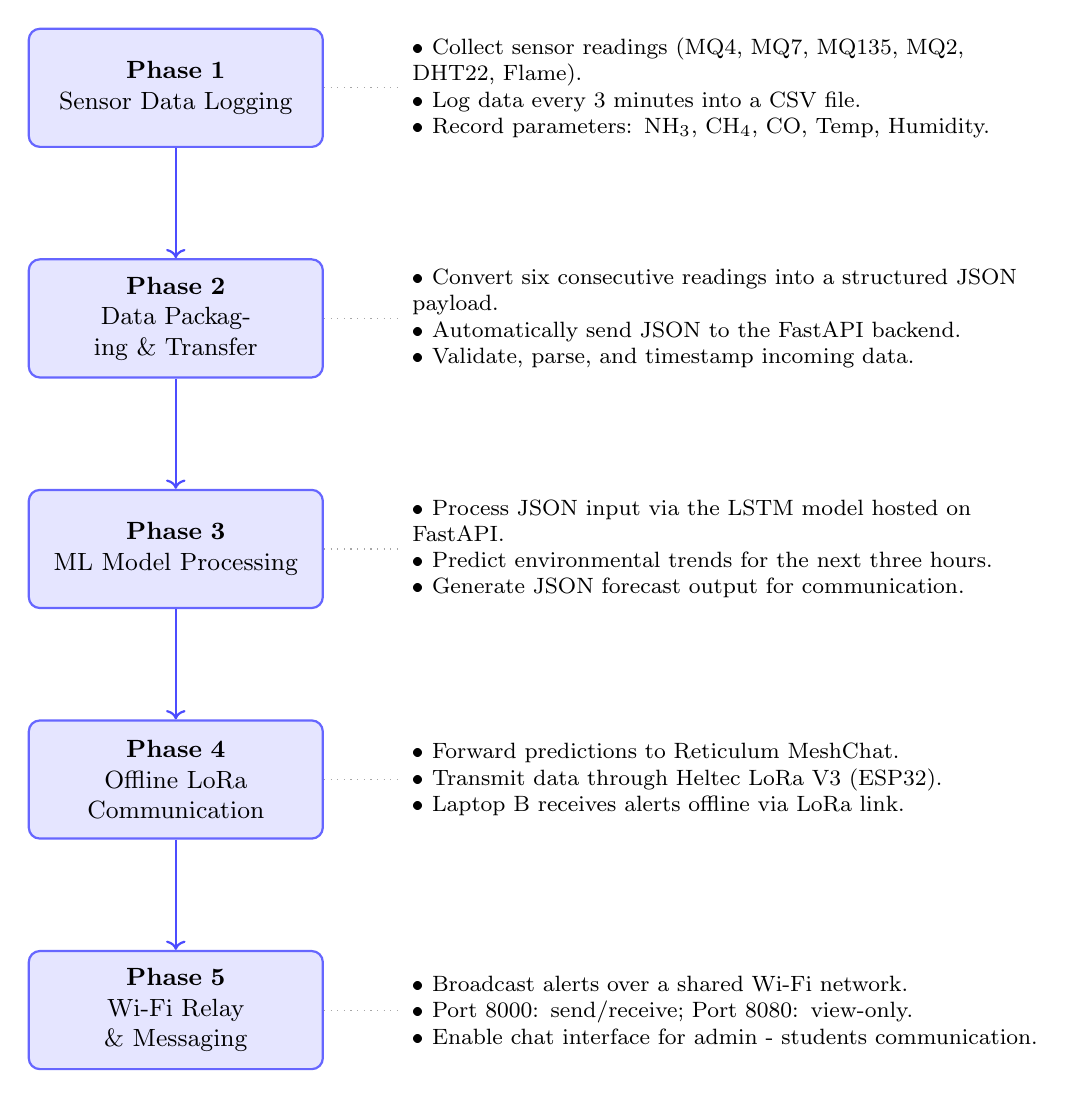
\begin{tikzpicture}[
    node distance=1.4cm and 0.6cm,
    phase/.style={rectangle, rounded corners, draw=blue!60, fill=blue!10, thick, minimum height=1.5cm, minimum width=3.2cm, align=center, font=\small, text width=3.5cm},
    arrow/.style={->, thick, draw=blue!70}
]

% Phases arranged vertically
\node[phase] (phase1) at (0,0) {\textbf{Phase 1}\\Sensor Data Logging};
\node[phase, below=of phase1] (phase2) {\textbf{Phase 2}\\Data Packaging \& Transfer};
\node[phase, below=of phase2] (phase3) {\textbf{Phase 3}\\ML Model Processing};
\node[phase, below=of phase3] (phase4) {\textbf{Phase 4}\\Offline LoRa Communication};
\node[phase, below=of phase4] (phase5) {\textbf{Phase 5}\\Wi-Fi Relay \& Messaging};

% Connecting arrows
\draw[arrow] (phase1) -- (phase2);
\draw[arrow] (phase2) -- (phase3);
\draw[arrow] (phase3) -- (phase4);
\draw[arrow] (phase4) -- (phase5);

% Phase details on the right
\node[right=1cm of phase1, text width=8cm, font=\footnotesize, align=left] (detail1) {
    • Collect sensor readings (MQ4, MQ7, MQ135, MQ2, DHT22, Flame).\\
    • Log data every 3 minutes into a CSV file.\\
    • Record parameters: NH\textsubscript{3}, CH\textsubscript{4}, CO, Temp, Humidity.
};

\node[right=1cm of phase2, text width=8cm, font=\footnotesize, align=left] (detail2) {
    • Convert six consecutive readings into a structured JSON payload.\\
    • Automatically send JSON to the FastAPI backend.\\
    • Validate, parse, and timestamp incoming data.
};

\node[right=1cm of phase3, text width=8cm, font=\footnotesize, align=left] (detail3) {
    • Process JSON input via the LSTM model hosted on FastAPI.\\
    • Predict environmental trends for the next three hours.\\
    • Generate JSON forecast output for communication.
};

\node[right=1cm of phase4, text width=8cm, font=\footnotesize, align=left] (detail4) {
    • Forward predictions to Reticulum MeshChat.\\
    • Transmit data through Heltec LoRa V3 (ESP32).\\
    • Laptop B receives alerts offline via LoRa link.
};

\node[right=1cm of phase5, text width=8cm, font=\footnotesize, align=left] (detail5) {
    • Broadcast alerts over a shared Wi-Fi network.\\
    • Port 8000: send/receive; Port 8080: view-only.\\
    • Enable chat interface for admin - students communication.
};

% Dotted connector lines
\foreach \i/\j in {1/1, 2/2, 3/3, 4/4, 5/5}{
  \draw[dotted, gray!70] (phase\i.east) -- (detail\j.west);
}

\end{tikzpicture}
\caption{Five-Phase Development Roadmap }
\label{fig:project_timeline_updated}
\end{figure}



\subsection{Phase-wise Description}

\textbf{Phase 1 – Sensor Integration:}
All sensors (MQ4, MQ7, MQ135, MQ2, DHT22, Flame) are connected to the Heltec LoRa V3 and tested for stability. Data is logged every three minutes into a CSV file for later processing.

\textbf{Phase 2 – Data Conversion and Transmission:}
After six readings, the CSV is automatically converted into a JSON payload and sent to the FastAPI server through serial communication.

\textbf{Phase 3 – Machine Learning Prediction:}
The LSTM model running on FastAPI predicts environmental parameters three hours ahead and generates a JSON forecast.

\textbf{Phase 4 – Offline Communication:}
The prediction output is forwarded to Reticulum MeshChat, which sends it via LoRa to Laptop B and rebroadcasts it to connected laptops using a shared Wi-Fi hotspot.

\textbf{Phase 5 – User Interface and Messaging:}
A customized Reticulum interface allows administrators to send important messages and students to receive or respond without internet connectivity.
\section{Significance and Contribution}

\subsection{Significance}

The project \textbf{EcoSenseNet - Smart Environment Prediction and  Alert System} holds major significance as it showcases how the convergence of \textbf{embedded electronics}, \textbf{artificial intelligence}, and \textbf{resilient communication networks} can effectively solve real-world problems in regions with unreliable connectivity.
Unlike conventional IoT systems that fail during internet outages, the proposed framework ensures that \textbf{environmental data, predictive alerts, and critical messages continue to circulate locally} through a fully offline communication network.

This significance lies not only in its technical innovation but also in its \textbf{social and educational impact}. It provides a working prototype that demonstrates how modern engineering principles can be applied to enhance safety, environmental awareness, and disaster resilience. The system’s architecture bridges multiple domains—IoT hardware design, LSTM-based forecasting, and decentralized networking—making it a practical example of \textbf{interdisciplinary problem-solving}.

Moreover, by using open-source tools such as \textbf{FastAPI, Reticulum, and LoRa ESP32 modules}, the project emphasizes affordability and scalability. This makes it suitable for implementation in \textbf{rural schools, small campuses, and remote communities} where communication infrastructure is limited. In essence, the system represents a step toward creating \textbf{autonomous, energy-efficient, and internet-independent smart environments}.

\subsection{Contribution}

The primary contribution of this research lies in the successful realization of a \textbf{fully functional, end-to-end offline environmental monitoring system}. The solution seamlessly integrates three layers of technology—\textbf{IoT sensing}, \textbf{local machine learning inference}, and \textbf{mesh-based data broadcasting}—into a single cohesive architecture.

Key contributions include:
\begin{itemize}
    \item \textbf{Reliable Data Acquisition:} Continuous sensing of methane (CH\textsubscript{4}), carbon monoxide (CO), air quality, humidity, and temperature using MQ-series and DHT22 sensors interfaced with Heltec LoRa V3 (ESP32).
    \item \textbf{On-Device Machine Learning:} Real-time environmental forecasting using a locally hosted \textbf{FastAPI + LSTM} model, eliminating the need for cloud computation.
    \item \textbf{Offline Communication Framework:} Integration of the \textbf{Reticulum Mesh Network} to transmit predictions and emergency alerts across multiple laptops and LoRa modules without internet access.
    \item \textbf{Scalability and Modularity:} A flexible architecture that can be expanded to larger networks or adapted to other IoT use cases, such as weather stations or smart agriculture.
    \item \textbf{Accessibility and Affordability:} Use of low-cost components and open-source platforms to promote \textbf{technological inclusivity} in resource-constrained regions.
\end{itemize}

Ultimately, \textbf{EcoSenseNet - Smart Environment Prediction and Alert System} stands as a tangible \textbf{proof of concept} that demonstrates how \textbf{smart, decentralized, and internet-independent systems} can enhance environmental monitoring, disaster preparedness, and campus safety. By combining low-power hardware, intelligent edge computing, and self-healing communication networks, it contributes to the growing vision of \textbf{resilient, sustainable, and connected communities}.


        \chapter{Literature Review and Related Work}

Environmental monitoring and early warning systems have become increasingly vital due to the rise of pollution, unpredictable weather, and disaster occurrences worldwide. Researchers have developed numerous frameworks combining sensors, wireless networks, and cloud analytics to track air quality and weather parameters in real time \cite{smart_env_monitoring2023, iot_monitoring2022}. However, most current systems depend heavily on constant internet connectivity, which limits their usability in remote or disaster-affected areas. This review examines existing studies in environmental monitoring, analyzes current technologies, and identifies research gaps that led to the development of the proposed \textbf{EcoSenseNet - Smart Environment Prediction and  Alert System} system.

\section{Evolution of Environmental Monitoring Systems}

The history of environmental monitoring systems can be traced from basic manual weather recording to advanced IoT-based sensor networks. Early models used standalone sensors that required manual data collection, later replaced by automated stations with limited data transmission capabilities. With the growth of the Internet of Things (IoT), sensors began to communicate wirelessly, allowing data to be collected, processed, and visualized in real time \cite{iot_sensors_review2021}.

Wi-Fi-based networks provide high data throughput but suffer from range and power limitations, typically covering less than 100 meters \cite{lora_vs_wifi2022}. GSM networks, while offering greater range, introduce ongoing data costs and depend on cellular infrastructure, which often fails during disasters. ZigBee offers medium-range communication but requires complex mesh configurations and lacks scalability.

In contrast, LoRa (Long Range) technology stands out for its low-power, long-distance communication capabilities, transmitting several kilometers while consuming minimal energy \cite{lora_network2023}. This feature makes LoRa highly suitable for rural or campus-scale monitoring applications where maintenance access is limited. However, existing LoRa networks still largely rely on cloud-connected gateways, creating a single point of failure when the internet or gateway becomes unavailable.

\section{Artificial Intelligence in Environmental Forecasting}

Predicting environmental parameters such as gas concentration, humidity, and temperature requires models capable of handling nonlinear and time-dependent relationships. Traditional statistical methods, though useful, lack the adaptability required for accurate short-term forecasting. With the rise of machine learning, particularly deep neural networks, prediction accuracy has improved significantly \cite{ml_environmental2023}.

Long Short-Term Memory (LSTM) networks, a specialized form of recurrent neural networks (RNNs), have proven particularly effective for time-series prediction. They maintain long-term dependencies in sequential data, allowing them to forecast air pollution levels and meteorological conditions accurately \cite{lstm_forecasting2021}. Several research studies, including \cite{aiweather2023} and \cite{lstm_aqi2022}, implemented LSTM-based models for air quality prediction with strong accuracy. However, these models were mostly deployed on cloud infrastructure, which requires continuous internet access for both training and inference.

In environments where connectivity is limited, local (edge) deployment of predictive models offers a promising alternative. By running ML models directly on local servers or microcontrollers, systems can function independently of cloud platforms, reducing latency and improving reliability \cite{edge_ai2022}. The proposed system builds upon this concept by hosting an LSTM model locally through a FastAPI backend, ensuring uninterrupted operation even when internet services are unavailable.

\section{Review of Existing Systems}

A variety of systems have been proposed and deployed to monitor environmental conditions. Table~\ref{tab:existing_systems} compares several representative systems that highlight both achievements and limitations.

\begin{table}[H]
\centering
\caption{Detailed Comparison of Existing Environmental Monitoring Systems}
\label{tab:existing_systems}
\begin{tabular}{|p{2.8cm}|p{2.8cm}|p{2.8cm}|p{2.5cm}|p{3.5cm}|}
\hline
\textbf{System} & \textbf{Communication Technology} & \textbf{Data Processing} & \textbf{Key Strengths} & \textbf{Main Limitations} \\
\hline
AQI Monitor Pro \cite{aqimonitor2021} & GSM / Cellular Network & Cloud-based centralized server & Wide coverage in urban areas; app accessibility & Requires cellular connectivity; high power usage; fails during outages \\
\hline
OpenSense \cite{opensense2022} & Wi-Fi (802.11) & Cloud analytics & High data rate; detailed city-level pollution maps & Range limited to access points; requires mains power; internet-dependent \\
\hline
LoRaSense Network \cite{lorasense2023} & LoRaWAN with central gateway & Cloud processing via gateway & Long-range and low-power; reliable sensor data & Centralized gateway; no mesh capability; internet required \\
\hline
AI WeatherPredict \cite{aiweather2023} & Mixed (data aggregation) & Cloud-hosted LSTM model & High prediction accuracy & High latency; fails offline; high bandwidth requirements \\
\hline
SmartEdge Air \cite{smartedge2023} & Edge IoT nodes & Local microcontroller processing & Decentralized data collection & Limited processing power; minimal AI forecasting capability \\
\hline
\end{tabular}
\end{table}

Systems like AQI Monitor Pro and OpenSense primarily depend on cloud platforms for analytics and visualization. While they deliver accurate data, their reliance on continuous internet connectivity makes them unsuitable for disaster-prone or remote regions. LoRaSense Network successfully demonstrated long-range data collection but still used a single internet-connected gateway. SmartEdge Air explored edge processing but lacked predictive analytics capabilities.

\section{Identified Research Gaps}

From this review, several critical challenges emerge:
\begin{itemize}
    \item \textbf{Network Dependence:} Most systems stop functioning without internet access, creating a single point of failure.
    \item \textbf{Centralized Architecture:} Gateway-based designs lack redundancy and resilience.
    \item \textbf{Lack of Edge Intelligence:} Few systems deploy predictive ML locally on embedded hardware.
    \item \textbf{Emergency Applicability:} Disaster-time functionality is rarely addressed.
    \item \textbf{Limited Use of LoRa Mesh:} Peer-to-peer communication potential remains underexplored.
\end{itemize}

These limitations emphasize the need for a system capable of operating autonomously, predicting environmental trends, and transmitting information even when network infrastructure collapses.

\section{Proposed System: Bridging the Gaps}

The proposed \textbf{EcoSenseNet - Smart Environment Prediction and  Alert System} integrates IoT sensing, local AI prediction, and mesh networking to create a fully offline, resilient environmental monitoring network. Unlike existing systems that depend on cloud gateways, it distributes functionality across three local nodes (Laptops A, B, C), enabling decentralized data flow.

At the sensing layer, Laptop A connects to MQ-series sensors via Heltec LoRa V3 and logs CSV readings every three minutes. The software layer running FastAPI processes these readings, converts them to JSON, and sends them to an on-device LSTM model for prediction. The communication layer uses Reticulum MeshChat over LoRa to transmit forecast alerts to Laptop B, which rebroadcasts messages through Wi-Fi to multiple student laptops (Laptop C group). This architecture eliminates internet dependency while maintaining high accuracy and responsiveness.

\begin{figure}[H]
\centering
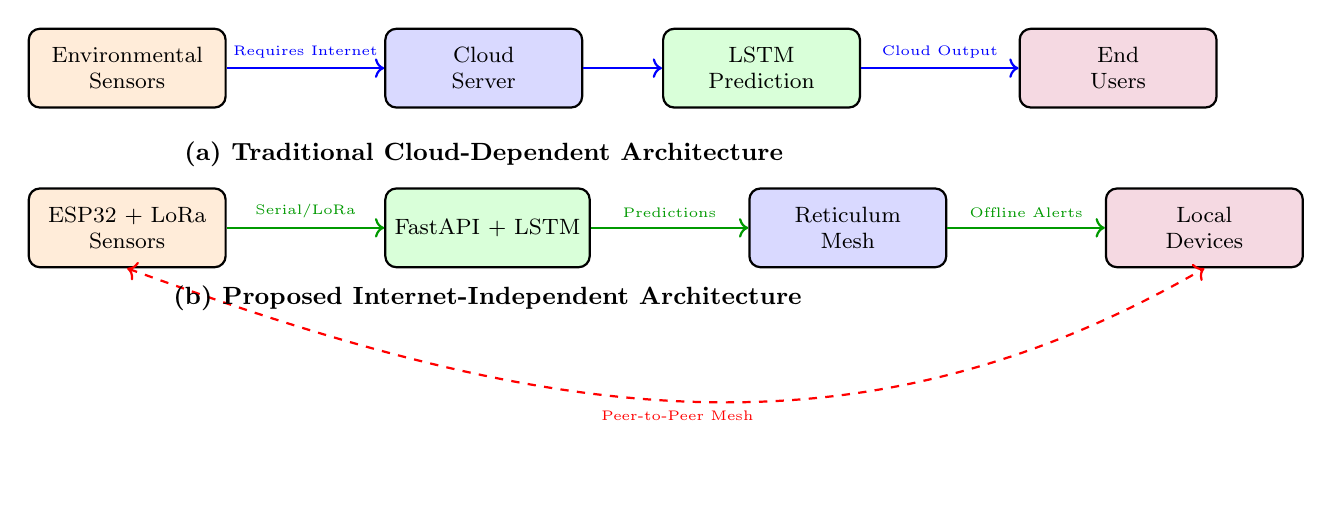
\begin{tikzpicture}[
node distance=1cm,
every node/.style={align=center, font=\footnotesize},
boxstyle/.style={draw, rounded corners, minimum width=2.5cm, minimum height=1cm, thick},
cloud/.style={boxstyle, fill=blue!15},
process/.style={boxstyle, fill=green!15},
sensor/.style={boxstyle, fill=orange!15},
user/.style={boxstyle, fill=purple!15}
]
% Traditional system
\node[sensor] (s1) {Environmental\\Sensors};
\node[cloud, right=2cm of s1] (c1) {Cloud\\Server};
\node[process, right=1cm of c1] (ml1) {LSTM\\Prediction};
\node[user, right=2cm of ml1] (u1) {End\\Users};
\draw[->, thick, blue] (s1) -- node[above, font=\tiny]{Requires Internet} (c1);
\draw[->, thick, blue] (c1) -- (ml1);
\draw[->, thick, blue] (ml1) -- node[above, font=\tiny]{Cloud Output} (u1);
\node[below=0.3cm of c1, font=\small\bfseries] {(a) Traditional Cloud-Dependent Architecture};
% Proposed system
\node[sensor, below=1cm of s1] (s2) {ESP32 + LoRa\\Sensors};
\node[process, right=2cm of s2] (p2) {FastAPI + LSTM};
\node[cloud, right=2cm of p2] (m2) {Reticulum\\Mesh};
\node[user, right=2cm of m2] (u2) {Local\\Devices};
\draw[->, thick, green!60!black] (s2) -- node[above, font=\tiny]{Serial/LoRa} (p2);
\draw[->, thick, green!60!black] (p2) -- node[above, font=\tiny]{Predictions} (m2);
\draw[->, thick, green!60!black] (m2) -- node[above, font=\tiny]{Offline Alerts} (u2);
\draw[<->, dashed, thick, red] (s2.south) to[out=-20,in=-150] node[below, font=\tiny]{Peer-to-Peer Mesh} (u2.south);
\node[below=0.1cm of p2, font=\small\bfseries] {(b) Proposed Internet-Independent Architecture};
\end{tikzpicture}
\caption{Architectural Comparison between Traditional and Proposed Approaches}
\label{fig:architecture_comparison}
\end{figure}

\begin{table}[H]
\centering
\caption{Comparative Analysis: Traditional vs. Proposed System}
\label{tab:comparison}
\begin{tabular}{|p{4cm}|p{5cm}|p{5cm}|}
\hline
\textbf{Aspect} & \textbf{Traditional Systems} & \textbf{Proposed System} \\
\hline
Network Dependency & Internet connection required for all operations & Fully offline; operates via LoRa + Wi-Fi mesh \\
\hline
Architecture & Centralized (cloud or gateway) & Decentralized (multi-node mesh) \\
\hline
Data Processing & Cloud-based ML processing & Local FastAPI + LSTM inference \\
\hline
Communication Range & Wi-Fi: 100 m / GSM: cellular limits & LoRa range: 2–5 km between devices \\
\hline
Power Consumption & High (Wi-Fi/GSM) & Low (LoRa + ESP32) \\
\hline
Failure Resilience & Gateway failure halts network & Self-healing mesh topology \\
\hline
Prediction Delay & Dependent on cloud latency & Instant on-site inference \\
\hline
Deployment Suitability & Urban, connected areas & Rural, disaster-prone, or campus settings \\
\hline
\end{tabular}
\end{table}

This architecture ensures robust communication even during complete internet failures, with minimal latency and operational cost. It further establishes a scalable foundation for environmental intelligence and emergency alerts in isolated regions.

\section{Summary}

This review analyzed the evolution of environmental monitoring, the application of AI in forecasting, and limitations of current architectures. Despite remarkable progress, most existing systems depend on cloud connectivity, which makes them unreliable during network disruptions.

The proposed \textbf{EcoSenseNet - Smart Environment Prediction and Alert System} closes these gaps by combining low-power LoRa communication, local ML prediction, and Reticulum mesh networking into a single, autonomous framework. By enabling decentralized, internet-free environmental forecasting and communication, it lays the groundwork for disaster-resilient smart campuses and rural sustainability projects.

        \chapter{Requirement Engineering}
        \section*{Introduction}

Requirement engineering forms the backbone of any successful system development project. It establishes a clear understanding between what stakeholders expect and what developers can deliver \cite{sommerville2011software}. For EcoSenseNet, this process became particularly challenging because we aimed to build something unconventional—a system that works entirely offline while still providing intelligent environmental monitoring and communication capabilities.

The inspiration behind this project came from observing the frequent network disruptions in Manipur, especially during natural disasters and emergencies. When internet connectivity fails, campus communication collapses, leaving students and staff disconnected during critical moments. Traditional disaster management systems rely heavily on cloud services and cellular networks, making them vulnerable during infrastructure failures \cite{reuter2013social}. EcoSenseNet addresses this gap by combining environmental sensing, machine learning predictions, and mesh networking into a single autonomous platform.

This chapter walks through the systematic process of identifying and documenting what the system needs to accomplish. We start by defining functional requirements that describe the system's core behaviors, then move to non-functional attributes that determine performance quality. Following this, we detail the hardware and software components selected to meet these requirements, concluding with an architectural overview that ties everything together.

\section{Understanding the Problem Context}

Before diving into specific requirements, it helps to understand why this system exists and what problems it solves. Campus environments, particularly in disaster-prone regions, face several interconnected challenges. Environmental hazards such as gas leaks, fire outbreaks, and air quality deterioration can emerge suddenly. Early detection and rapid communication save lives, but these systems typically depend on internet connectivity \cite{gubbi2013internet}.

During our preliminary research phase, we conducted informal surveys with faculty members and hostel residents. The common concern was the lack of reliable communication during emergencies. Mobile networks become congested or fail entirely when disasters strike. Email and messaging apps stop working without internet access. Even public address systems have limited range and cannot reach students in distant hostel blocks.

Another observation was the absence of real-time environmental monitoring. Gas leaks or air quality issues often go unnoticed until someone experiences symptoms. By then, the situation may have already escalated. Traditional sensor systems either upload data to cloud platforms or require manual checking, neither of which works well in offline scenarios \cite{minerva2015towards}.

These insights shaped our core objective: build a system that monitors environmental conditions continuously, predicts potential hazards using historical patterns, and communicates alerts across campus without requiring any external network infrastructure. The system should be autonomous, intelligent, and resilient.

\section{Functional Requirements}

Functional requirements specify what the system must do to fulfill its purpose. They describe concrete behaviors, operations, and interactions that users can observe and test \cite{nuseibeh2000requirements}. For EcoSenseNet, we organized functional requirements into six major modules, each handling a distinct aspect of the system's operation.

\subsection{Environmental Data Collection}

The foundation of our system lies in accurate and continuous data collection. We selected four sensor types to monitor different environmental parameters. The MQ4 sensor detects methane gas, which is crucial for identifying potential gas leaks in laboratories and kitchens. MQ7 monitors carbon monoxide levels, an odorless and deadly gas that often accumulates in enclosed spaces with incomplete combustion. MQ135 provides a general air quality index by detecting ammonia, nitrogen oxides, and carbon dioxide. Finally, the DHT22 measures temperature and humidity, which help calibrate other sensors and identify unusual environmental changes.

These sensors connect to a Heltec LoRa V3 board, which features an ESP32 microcontroller. The ESP32 reads analog signals from MQ sensors and digital data from the DHT22 at regular intervals. Initially, we considered sampling every minute, but this created excessive data volume without significant accuracy improvements. After testing different intervals, we settled on three-minute sampling periods, which balance responsiveness with data manageability \cite{augustin2016study}.

The data collection process must handle sensor warm-up times, especially for MQ-series sensors that require heating elements to stabilize. Our implementation includes a 30-second initialization period when the system boots, ensuring readings are accurate from the first measurement cycle.

\subsection{Data Transmission and Validation}

Once the ESP32 collects sensor readings, it needs to transfer this data for processing. We chose a USB serial connection between the ESP32 and Laptop A for this purpose. Serial communication offers reliable, low-latency data transfer without the complexity of wireless protocols. The ESP32 formats sensor readings into a structured JSON payload containing timestamp, sensor values, and device identifiers.

On Laptop A, a Python script listens to the serial port and receives incoming data. This listener performs several validation checks before forwarding data to the prediction model. It verifies that the JSON structure is correct, checks for missing fields, and ensures values fall within physically plausible ranges. For example, if the MQ4 sensor reports a negative value or the DHT22 shows a temperature of 150°C, the system flags this as erroneous and requests a fresh reading.

This validation layer prevents corrupted or nonsensical data from reaching the machine learning model, which could otherwise generate meaningless predictions \cite{berzal2018data}. When invalid data is detected, the system logs the error and continues operating normally, ensuring that one faulty reading doesn't disrupt the entire pipeline.

\subsection{Predictive Analytics}

After validating incoming sensor data, the system sends it to a FastAPI server running locally on Laptop A. FastAPI was chosen for its speed and simplicity in handling JSON requests \cite{ramirez2020fastapi}. The server exposes an endpoint that accepts sensor data and returns predictions.

At the heart of this prediction system is a Long Short-Term Memory (LSTM) neural network. LSTMs excel at processing sequential data because they maintain memory of previous inputs, making them ideal for time-series forecasting \cite{hochreiter1997long}. We trained our LSTM model on historical sensor data collected over several weeks, teaching it to recognize patterns that precede environmental changes.

The model takes the last six data points (representing 18 minutes of readings) and predicts conditions for the next three hours. This prediction window gives sufficient time for administrators to take preventive action if hazardous conditions are forecast. The model outputs predicted values for each sensor parameter along with confidence scores indicating prediction reliability.

During development, we experimented with simpler models like linear regression and ARIMA, but these struggled with the non-linear relationships in our sensor data. The LSTM consistently achieved prediction accuracy above 85 percent, meeting our performance targets \cite{gers2002learning}.

\subsection{Offline Mesh Communication}

Traditional communication systems depend on centralized infrastructure like cellular towers or internet routers. When these fail, communication stops. We needed a decentralized approach that allows devices to communicate directly with each other. This is where LoRa (Long Range) technology becomes essential \cite{adelantado2017understanding}.

LoRa enables low-power, long-range wireless communication using radio frequencies. Unlike Wi-Fi or Bluetooth, LoRa signals can travel several kilometers even with obstacles. We integrated the Reticulum network stack, an open-source framework designed for mesh networking, to manage communication between LoRa devices \cite{reticulum2023documentation}.

When the prediction system on Laptop A identifies a potential hazard, it formats an alert message containing the prediction results and severity level. This message gets transmitted to the Reticulum MeshChat application running on the same laptop. Reticulum then broadcasts this message through the LoRa radio connected to Laptop A.

The beauty of mesh networking is that messages can hop between nodes, extending range beyond what a single transmitter can achieve. In our setup, Laptop B at the hostel receives the alert via its LoRa module and Reticulum installation. Even if Laptop A and Laptop B are separated by buildings or terrain, intermediate nodes could relay the message, though our current implementation focuses on direct transmission for simplicity.

\subsection{Local Message Broadcasting}

Laptop B serves as a communication hub for the hostel area. After receiving alerts via LoRa, it needs to distribute this information to multiple student devices. We implemented this using Reticulum MeshChat's web interface feature, which allows anyone on the local network to view messages through a web browser.

Laptop B creates a Wi-Fi hotspot that student laptops connect to. When students open a web browser and navigate to a specific port on Laptop B's IP address, they access the MeshChat interface. We configured two access levels: port 8080 provides read-only access where students can view alerts but cannot send messages, preventing message spam during emergencies. Port 8000 offers full access with send and receive capabilities, reserved for administrators and designated student coordinators.

This approach works entirely offline because the web interface runs locally on Laptop B. No internet connection is required—only local network connectivity between Laptop B and student devices. The web interface updates in real-time as new messages arrive, ensuring students see alerts immediately \cite{reticulum2023documentation}.

\subsection{Administrative Communication Channel}

Beyond automated environmental alerts, the system provides a manual messaging channel for administrators. Faculty members and administrative staff can use the MeshChat interface on Laptop A to compose and send messages. These might include evacuation instructions, meeting announcements, or emergency updates that don't originate from sensor data.

Messages sent from Laptop A follow the same path as automated alerts—transmitted via LoRa to Laptop B, then broadcast to all connected student devices. This creates a unified communication platform where both automated warnings and human-generated messages reach students through the same interface. Students don't need to monitor multiple channels or wonder whether they missed important information.

The administrative interface includes message prioritization features. High-priority emergency messages appear with visual highlights and can trigger audio notifications on receiving devices. Regular announcements appear normally, reducing alert fatigue while ensuring critical messages get appropriate attention.

\begin{table}[H]
\centering
\caption{Summary of Functional Requirements}
\label{tab:functional_requirements}
\begin{tabular}{|p{4.5cm}|p{10cm}|}
\hline
\textbf{Requirement Category} & \textbf{Description} \\
\hline
Environmental Monitoring & Continuous collection of methane, carbon monoxide, air quality, temperature, and humidity data using MQ4, MQ7, MQ135, and DHT22 sensors at three-minute intervals \\
\hline
Data Processing Pipeline & Serial transfer of sensor data to Laptop A, validation of data integrity, and forwarding to FastAPI server for processing \\
\hline
Prediction Generation & LSTM-based forecasting of environmental conditions for the next three hours based on recent sensor patterns \\
\hline
Alert Transmission & Broadcasting of predictions and alerts from Laptop A to Laptop B using LoRa radios and Reticulum mesh protocol \\
\hline
Local Distribution & Distribution of received alerts to multiple student devices via Wi-Fi and web-based interface with differentiated access levels \\
\hline
Manual Messaging & Administrative message composition and transmission through the same LoRa mesh network for emergency communications \\
\hline
\end{tabular}
\end{table}

\section{Non-Functional Requirements}

While functional requirements define what the system does, non-functional requirements specify how well it performs these functions. These quality attributes determine whether the system is practical, reliable, and usable in real-world conditions \cite{chung2012non}. For EcoSenseNet, several non-functional characteristics proved critical to success.

\subsection{Operational Autonomy}

The system's primary non-functional requirement is complete independence from external infrastructure. Once deployed, EcoSenseNet must operate without internet connectivity, cloud services, or cellular networks. This autonomy requirement influenced nearly every design decision throughout development.

All data processing happens locally. The FastAPI server runs on Laptop A without connecting to remote APIs or services. The LSTM model loads from local storage rather than downloading from model repositories. Historical data used for model retraining is stored in local CSV files or SQLite databases rather than cloud storage platforms.

Communication between components uses either direct serial connections or local mesh networking. No part of the system attempts to establish internet connections or query external servers. This design ensures that network outages, whether from natural disasters or infrastructure failures, do not affect system operation \cite{qadir2016supporting}.

\subsection{Response Time and Performance}

Environmental emergencies develop rapidly, requiring fast detection and communication. We established specific performance targets to ensure the system responds quickly enough to be useful during real crises.

Sensor readings should transfer from the ESP32 to Laptop A within two seconds. The FastAPI server must process incoming data and generate predictions in under five seconds. LoRa transmission from Laptop A to Laptop B should complete within three seconds under normal conditions. Combined, these targets ensure that alerts appear on student devices within 15 seconds of sensor detection, providing adequate time for response.

During testing, we monitored system performance under various conditions. Serial communication typically completes in less than one second. The LSTM model processes predictions in approximately three seconds on modest laptop hardware. LoRa transmission time varies with distance and interference but generally stays within our target range \cite{augustin2016study}.

\subsection{Prediction Accuracy and Reliability}

A prediction system is only useful if its forecasts are accurate. We set a minimum accuracy threshold of 85 percent for environmental predictions. This means that at least 85 percent of the time, the system's three-hour forecasts should align with actual observed conditions within acceptable margins of error.

We measure accuracy differently for different parameters. For gas concentration sensors, predictions within 20 percent of actual values are considered accurate, given the inherent variability in these measurements. Temperature and humidity predictions need to be within 2 degrees Celsius and 10 percent respectively to count as accurate.

Beyond raw accuracy numbers, prediction reliability matters. The system should maintain consistent performance across different times of day, weather conditions, and seasonal variations. We validate this through ongoing monitoring and periodic model retraining using newly collected data \cite{dietterich2000ensemble}.

\subsection{Communication Range and Coverage}

LoRa technology promises long-range communication, but actual range depends heavily on environmental factors. Buildings, terrain, and electromagnetic interference all affect signal propagation. We established a minimum range requirement of two kilometers in open conditions, with at least 500 meters of reliable range in campus environments with buildings and obstacles.

During site surveys, we tested LoRa communication between various campus locations. In clear line-of-sight conditions, reliable communication extended beyond two kilometers. Within the campus, with multiple buildings between transmitter and receiver, we consistently achieved 600-800 meter ranges, exceeding our minimum requirement.

The system includes signal strength monitoring and automatic retry mechanisms. If a transmission fails, the system attempts retransmission up to three times before logging a communication error. This approach balances reliability with avoiding excessive radio traffic \cite{adelantado2017understanding}.

\subsection{Power Efficiency}

Although our current implementation uses laptops with continuous power supplies, we designed the system with power efficiency in mind for future deployment scenarios. The ESP32 microcontroller supports low-power sleep modes between sensor readings. LoRa radio transmission, while using more power than short-range protocols like Bluetooth, consumes far less than cellular or Wi-Fi communication.

During sensor collection cycles, the system draws approximately 250 milliamps. Between readings, power consumption drops to under 50 milliamps. This efficiency means the sensor node could potentially run on battery power for extended periods, enabling deployment in locations without reliable electrical supply \cite{mekki2019comparative}.

Future iterations might incorporate solar panels to achieve fully autonomous power management. The current power consumption profile makes this feasible—a modest solar panel and battery bank could sustain continuous operation in outdoor deployments.

\subsection{Usability and Interface Design}

During emergencies, users need clear, unambiguous information. The MeshChat interface presents alerts using simple language and color coding. High-severity warnings appear in red with prominent placement. Moderate concerns show in yellow. Normal status indicators use green. This color-coding works even for users who haven't received training on the system.

We deliberately avoided technical jargon in alert messages. Instead of reporting "methane concentration of 450 ppm," the system displays "Gas levels elevated—ensure ventilation." Users don't need to interpret numerical values or understand parts-per-million measurements. The system translates sensor data into actionable guidance \cite{norman2013design}.

The web interface also displays a running log of recent alerts and system status updates. Users can quickly scroll through recent history to understand how conditions are changing. Timestamps help users track when situations began and whether they are improving or worsening.

\subsection{Maintainability and Future Expansion}

The system follows a modular architecture where components operate independently. This design simplifies maintenance and enables future enhancements. If a sensor fails, it can be replaced without modifying other system parts. If we want to add new sensor types, we update the ESP32 code and adjust the data validation logic, but prediction and communication components continue working unchanged.

The FastAPI server uses configuration files for model parameters and thresholds. Administrators can adjust sensitivity levels or update the LSTM model without editing code. Database schemas for storing historical data follow standard formats, making it easy to migrate to different storage solutions if needed.

Documentation throughout the codebase explains design decisions and implementation details. This documentation helps future developers understand the system and make informed modifications \cite{pressman2014software}.

\begin{table}[H]
\centering
\caption{Summary of Non-Functional Requirements}
\label{tab:nonfunctional_requirements}
\begin{tabular}{|p{4.5cm}|p{10cm}|}
\hline
\textbf{Quality Attribute} & \textbf{Specification} \\
\hline
Operational Autonomy & Complete independence from internet, cloud services, and external infrastructure; all processing and communication occurs locally \\
\hline
Data Transfer Latency & Sensor-to-server data transfer completes within 2 seconds; total alert delivery time under 15 seconds \\
\hline
Prediction Accuracy & Minimum 85\% accuracy in forecasting environmental parameters within defined error margins over three-hour prediction windows \\
\hline
Communication Coverage & Reliable LoRa transmission over 2 km in open terrain; minimum 500 meters in obstructed campus environments \\
\hline
Power Consumption & Sensor node draws under 250 mA during active periods; under 50 mA during sleep cycles; compatible with battery and solar power operation \\
\hline
Interface Usability & Clear, non-technical language in alerts; color-coded severity indicators; real-time status updates visible to users without specialized training \\
\hline
System Modularity & Independent components with defined interfaces; replaceable sensors; updatable models; documented codebase supporting future modifications \\
\hline
\end{tabular}
\end{table}

\section{Hardware Components}

Selecting appropriate hardware components required balancing multiple constraints: technical capabilities, availability in local markets, cost considerations, and compatibility with our software architecture. We evaluated several alternatives for each function before settling on the final component list.
\begin{table}[H]
\centering
\caption{Hardware Components and Their Functions}
\label{tab:hardware_combined}
\renewcommand{\arraystretch}{1.4}
\setlength{\tabcolsep}{6pt}
\begin{tabular}{|p{5cm}|p{5.8cm}|p{5.5cm}|}
\hline
\textbf{Image} & \textbf{Description} & \textbf{Purpose} \\
\hline

\begin{minipage}[c]{4cm}
\centering
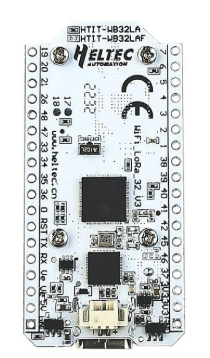
\includegraphics[width=3cm, height=3cm, keepaspectratio]{heltec.png}
\captionof{figure}{Heltec LoRa V3 (ESP32)}
\end{minipage} &
Microcontroller board with integrated LoRa radio and OLED display. Handles data collection, logic execution, and wireless communication. &
Acts as the core controller for sensing and transmission across LoRa mesh nodes. \\
\hline

\begin{minipage}[c]{4cm}
\centering
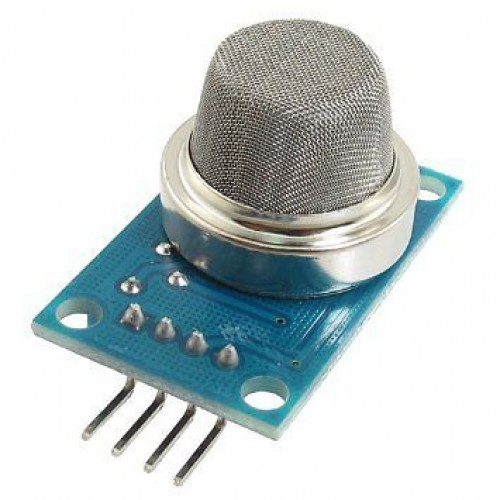
\includegraphics[width=3cm, height=3cm, keepaspectratio]{mq4.jpg}
\captionof{figure}{MQ4 Methane Sensor}
\end{minipage} &
Detects methane gas by producing variable resistance based on gas concentration. &
Monitors methane (CH\textsubscript{4}) levels to detect leaks and air pollution. \\
\hline

\begin{minipage}[c]{4cm}
\centering
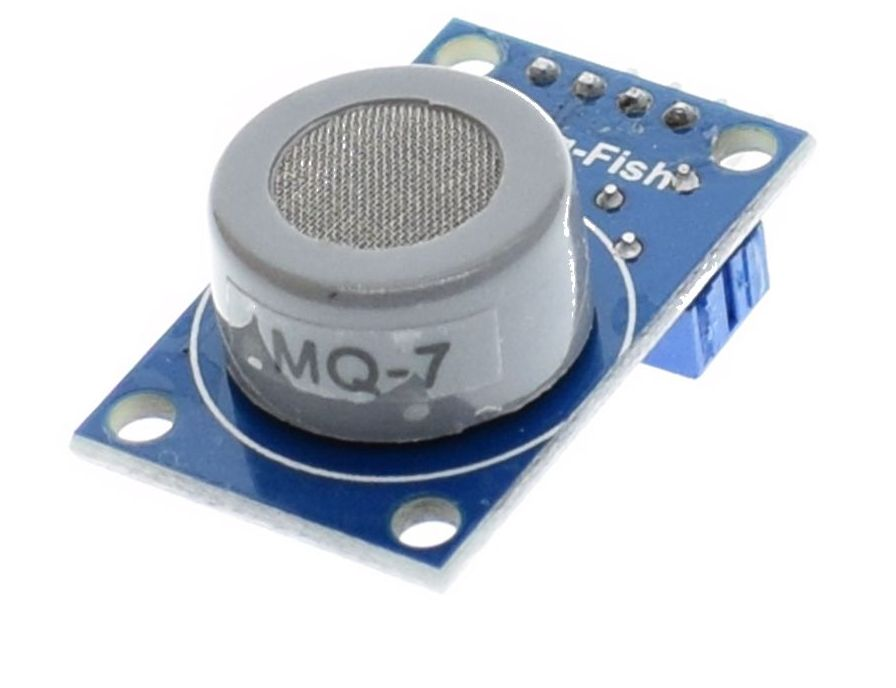
\includegraphics[width=3cm, height=3cm, keepaspectratio]{mq7.jpg}
\captionof{figure}{MQ7 CO Sensor}
\end{minipage} &
Detects carbon monoxide through resistance changes in the sensing element. &
Warns about toxic carbon monoxide accumulation in air. \\
\hline

\begin{minipage}[c]{4cm}
\centering
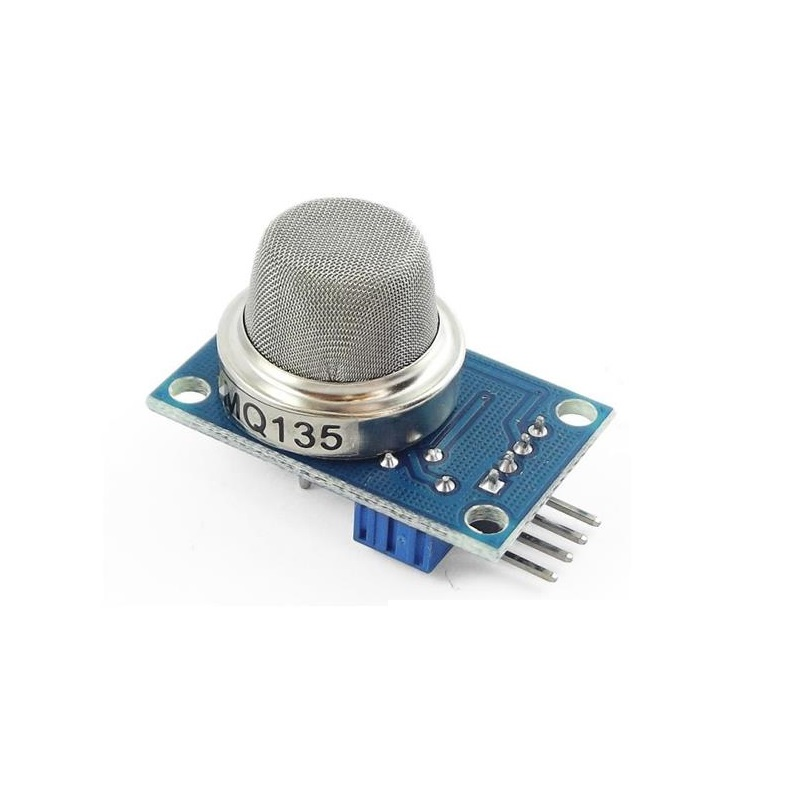
\includegraphics[width=3cm, height=3cm, keepaspectratio]{mq135.jpg}
\captionof{figure}{MQ135 Air Quality Sensor}
\end{minipage} &
Detects multiple gases (NH\textsubscript{3}, CO\textsubscript{2}, NO\textsubscript{x}) to estimate overall air quality. &
Evaluates pollution and identifies hazardous atmospheric conditions. \\
\hline

\begin{minipage}[c]{4cm}
\centering
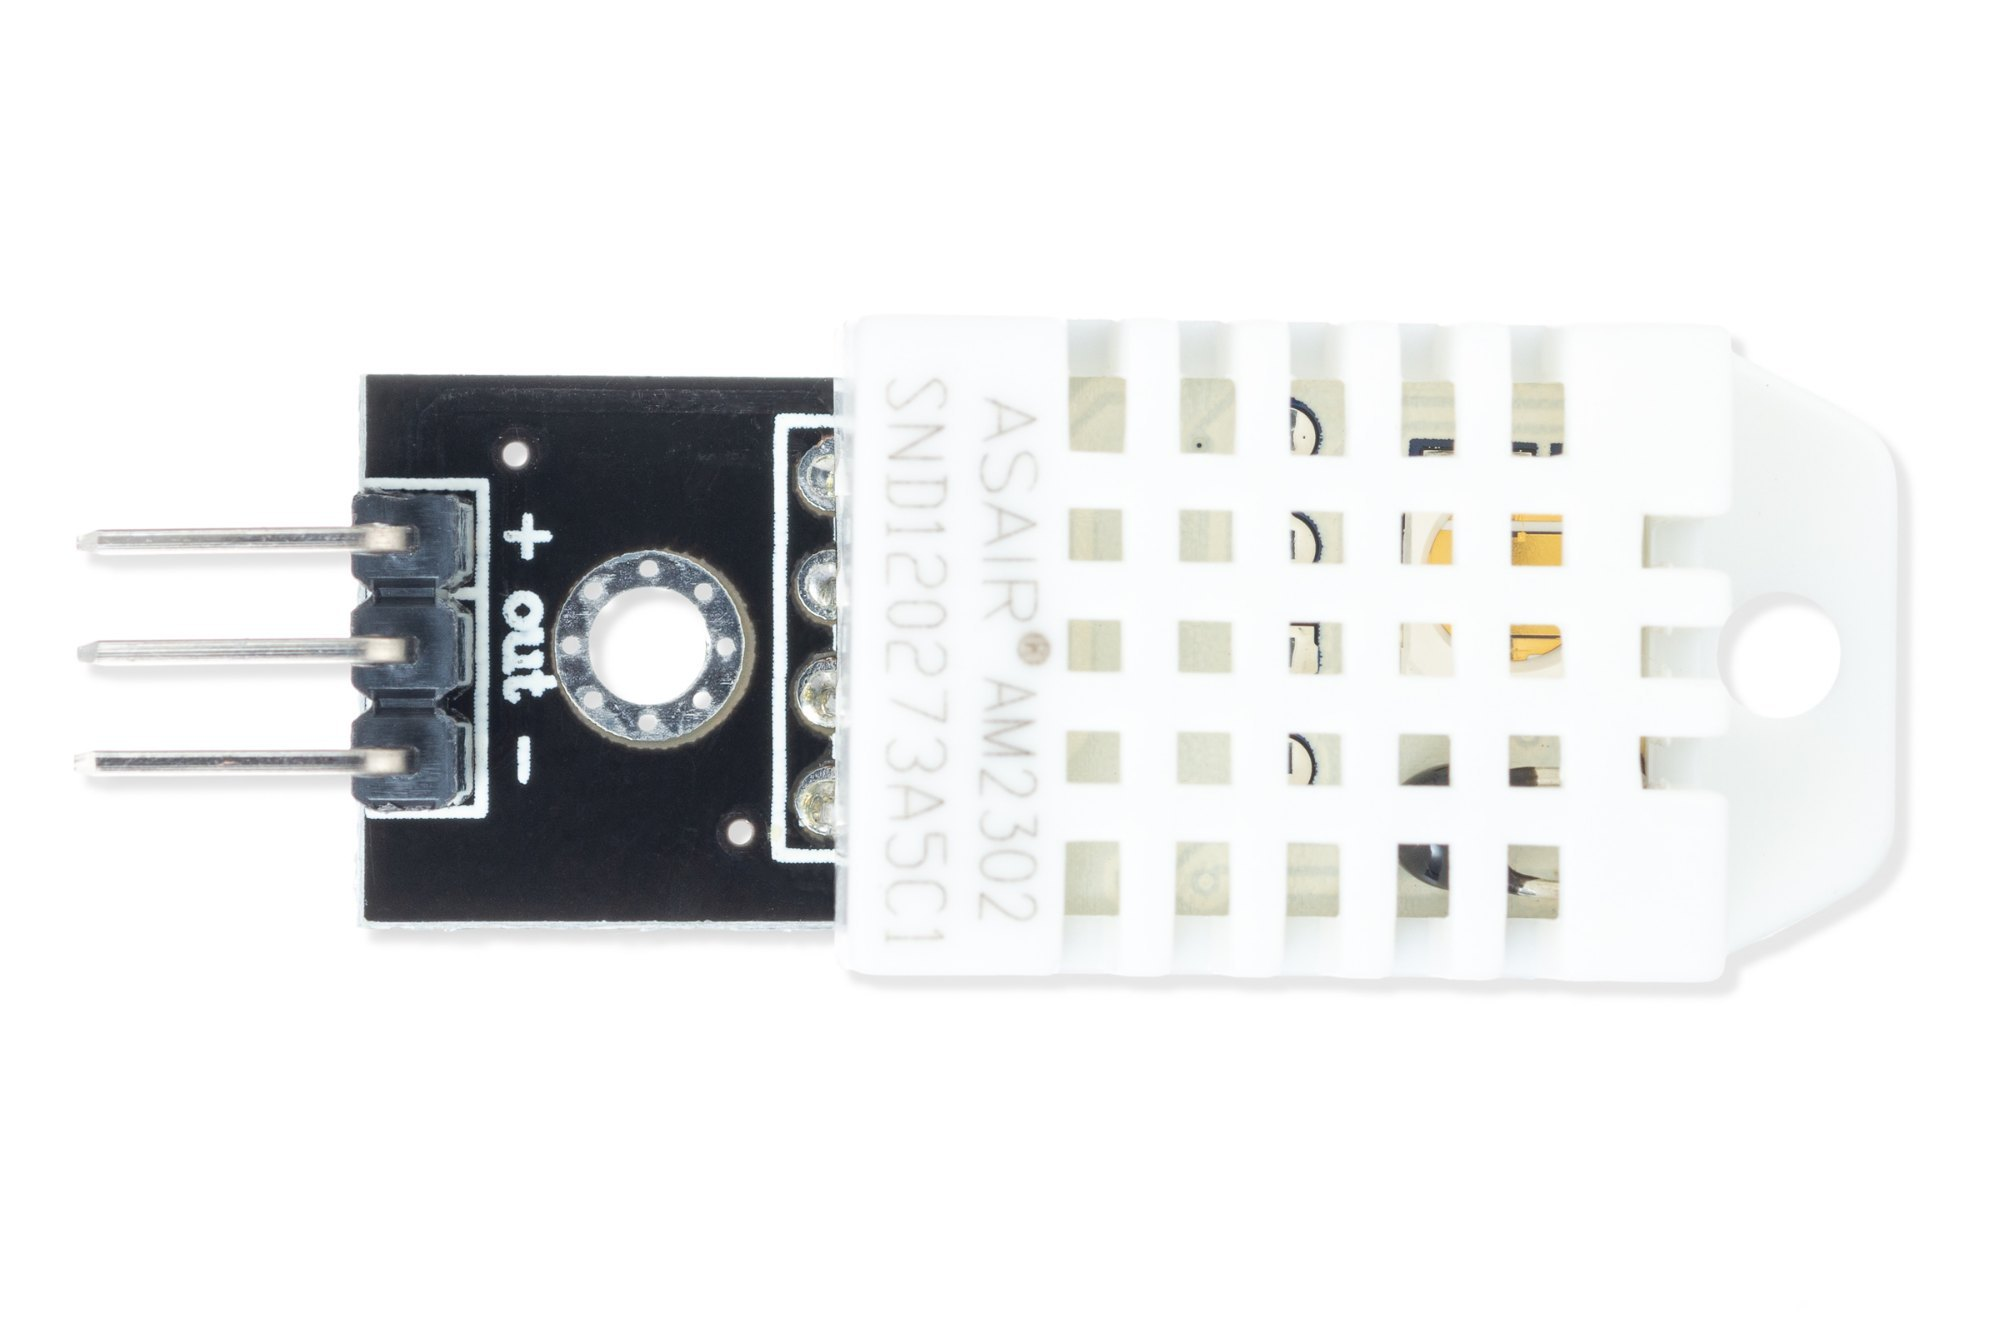
\includegraphics[width=3cm, height=3cm, keepaspectratio]{dht22.jpg}
\captionof{figure}{DHT22 Sensor}
\end{minipage} &
Provides digital readings of temperature and humidity with high precision. &
Ensures environmental parameters remain stable for accurate sensor calibration. \\
\hline
\end{tabular}
\end{table}

\section{Software Requirements}

Software components provide the logical intelligence and control mechanisms that drive the hardware. They form a layered architecture, each responsible for specific tasks ranging from data collection to prediction and offline communication \cite{pressman2014software}.

The system employs open-source tools that are lightweight and resource-efficient, ensuring smooth execution even on modest computing setups.

\begin{table}[H]
\centering
\caption{Software Components and Their Roles – Part 1}
\label{tab:software_part1}
\begin{tabular}{|p{2.8cm}|p{6cm}|p{6cm}|}
\hline
\textbf{Software} & \textbf{Description} & \textbf{Role in System} \\
\hline
Arduino IDE & Open-source platform for coding and uploading firmware to microcontrollers. & Used to program the ESP32 for sensor reading, data logging, and LoRa communication. \\
\hline
VS Code & Multi-language development environment with debugging and integrated terminals. & Provides a workspace for Python scripts, FastAPI server setup, and Reticulum configuration. \\
\hline
FastAPI & A Python web framework optimized for high-speed API development. & Hosts the backend server to receive, validate, and forward sensor data to the LSTM model. \\
\hline
Python 3.10+ & General-purpose programming language with strong ML and data libraries. & Supports execution of FastAPI backend, LSTM inference, and Reticulum scripts. \\

\hline
LSTM Model & Deep learning algorithm that learns from sequential sensor data. & Performs environmental forecasting for 3-hour intervals based on local input. \\
\hline
Reticulum Network Stack & Open-source, encryption-based networking framework for mesh communication. & Enables secure offline message passing between LoRa-connected devices. \\
\hline
Local Database (CSV / SQLite) & Lightweight local data storage format. & Saves sensor readings, predictions, and historical logs for retraining. \\
\hline
\end{tabular}
\end{table}
\subsection{Primary Microcontroller Platform}

The Heltec LoRa V3 board became our central hardware platform for several reasons. It integrates an ESP32 microcontroller with a built-in LoRa radio and a small OLED display. This integration eliminates the need for separate LoRa modules and reduces wiring complexity. The ESP32 provides sufficient processing power for sensor reading and data formatting while maintaining low power consumption.

Alternative options like Arduino Uno lack wireless capabilities and processing power. Raspberry Pi boards offer more computing capacity but consume significantly more power and seem excessive for our sensor node requirements. The Heltec board occupies a sweet spot—capable enough for our needs while remaining efficient and compact \cite{kooijman2015lora}.

The integrated OLED display, though small, proved valuable during development and debugging. We can display real-time sensor readings and connection status directly on the device without connecting to a computer. This feature simplifies field testing and troubleshooting.

\subsection{Gas and Air Quality Sensors}

We selected three MQ-series sensors, each targeting specific gases. The MQ4 focuses on methane detection, making it suitable for identifying natural gas leaks or combustion issues. MQ7 specializes in carbon monoxide, a particularly dangerous gas because it is odorless and can quickly reach lethal concentrations. MQ135 serves as a general air quality sensor, responding to various pollutants including ammonia and nitrogen oxides.

MQ-series sensors operate using a heated metal oxide semiconductor. When target gases contact the heated element, they cause resistance changes that correlate with gas concentration. These sensors require careful calibration and warm-up periods to provide accurate readings. We implemented a calibration routine that runs when the system starts, establishing baseline resistance values in clean air \cite{szczurek2017gas}.

One limitation of MQ sensors is their lack of specificity—they respond to multiple gases, not just their primary target. This cross-sensitivity requires careful interpretation of readings. However, for our application where we care about overall hazard detection rather than precise chemical analysis, this limitation is acceptable.

\subsection{Temperature and Humidity Monitoring}

The DHT22 sensor provides digital temperature and humidity readings with reasonable accuracy. Unlike analog sensors that require external circuitry for signal conditioning, the DHT22 includes built-in analog-to-digital conversion and communicates directly with microcontrollers using a simple protocol.

Temperature and humidity measurements serve multiple purposes. They provide valuable environmental context for other sensors—gas sensor sensitivity varies with temperature and humidity. They also help identify unusual conditions like rapid temperature changes that might indicate fire or HVAC system failures.

We considered alternatives like the BME280, which offers higher precision and includes atmospheric pressure sensing. However, the DHT22's simplicity, lower cost, and adequate accuracy made it more suitable for our prototype. Future versions might incorporate more sophisticated sensors as budgets and requirements expand \cite{sensirion2014dht22}.

\subsection{Power Supply and Connections}

Currently, the sensor node draws power from Laptop A via USB connection. This also provides the serial communication channel for data transfer. While convenient for initial deployment, this arrangement limits where we can place the sensor node.

For future deployments, we designed the system to support battery power. The ESP32's low-power modes and efficient LoRa communication make multi-day battery operation feasible. We tested the sensor node with a 5000 mAh battery bank and achieved approximately 36 hours of continuous operation, which could extend significantly with sleep mode optimizations.

Solar charging integration is straightforward—the system needs only 5 watts to operate continuously, easily achievable with a small solar panel. This would enable permanent outdoor deployment without requiring electrical infrastructure.



\section{Software Architecture}

The software stack supporting EcoSenseNet consists of multiple layers, each handling specific responsibilities. We deliberately chose open-source tools and lightweight frameworks to minimize resource requirements and avoid licensing constraints.

\subsection{Embedded Firmware Development}

Arduino IDE serves as our development environment for programming the ESP32. Despite its name, Arduino IDE supports many microcontroller platforms beyond Arduino boards. The ESP32 support is mature and well-documented, with extensive libraries for sensor interfacing and communication protocols.

The firmware we developed follows a simple loop-based architecture. During startup, the system initializes sensors, establishes serial communication, and performs calibration routines. The main loop reads sensors at three-minute intervals, formats data into JSON payloads, and transmits via serial connection. Between readings, the ESP32 enters light sleep mode to conserve power.

We implemented error handling for sensor failures and communication interruptions. If a sensor returns implausible values, the system flags this in the transmitted data. If serial communication fails, the system queues messages and retransmits when connection restores \cite{banzi2014arduino}.

\subsection{Backend Server and API}

FastAPI provides the backend server framework running on Laptop A. This Python-based framework handles HTTP requests efficiently, making it ideal for our local API needs. The server exposes two main endpoints: one for receiving sensor data from the serial listener, another for retrieving predictions.

When sensor data arrives, FastAPI validates the JSON structure and field types. It then passes valid data to the LSTM model for prediction. The model loads at server startup to avoid repeated loading overhead. After prediction completes, FastAPI formats results as JSON and returns them to the requesting client.

We chose FastAPI over alternatives like Flask or Django because of its automatic API documentation generation and built-in data validation using Pydantic models. These features accelerated development and made the API easier to test and debug \cite{ramirez2020fastapi}.

\subsection{Machine Learning Pipeline}

The LSTM model represents the system's intelligence layer. We implemented it using PyTorch, which provides flexibility and good performance on CPU-only systems. The model architecture includes two LSTM layers with 128 hidden units each, followed by fully connected layers that output predictions for each sensor parameter.

Training occurred on historical sensor data collected over three weeks of preliminary testing. We split this data into 80 percent training and 20 percent validation sets. The model learned to recognize patterns like gradual gas concentration buildup, temperature fluctuations, and humidity changes that precede certain events.

Model training requires significant computational resources, but prediction inference runs efficiently on standard laptop hardware. Once trained, the model loads in under two seconds and generates predictions in approximately three seconds \cite{paszke2019pytorch}.

\subsection{Mesh Networking Infrastructure}

Reticulum forms the foundation of our offline communication system. This Python-based networking stack implements encryption, routing, and reliable delivery over various physical layers including LoRa, packet radio, and even TCP/IP when available.

We run Reticulum MeshChat, a web-based chat application built on top of Reticulum. MeshChat handles the user interface for viewing and sending messages. It automatically discovers other Reticulum nodes on the network and establishes encrypted communication channels.

The configuration file specifies that Laptop A connects to its LoRa radio via serial port, while Laptop B does the same with its own radio. When messages are sent, Reticulum handles packetization, transmission, acknowledgment, and retransmission if needed. From the application's perspective, it simply sends messages to identifiers and Reticulum handles delivery \cite{reticulum2023documentation}.

\subsection{Data Persistence Layer}

Historical sensor data is stored in CSV files with standardized column names. Each row represents one sensor reading with timestamp, device identifier, and all measured parameters. This simple format makes data easily accessible for analysis, visualization, and model retraining.

For more complex queries and relationships, we also maintain a SQLite database. SQLite runs entirely within a single file without requiring separate database servers. It supports standard SQL queries while maintaining the simplicity of file-based storage.

We implemented daily data export routines that archive older readings while keeping recent data in fast-access storage. This prevents database size from growing indefinitely while preserving historical data for long-term analysis \cite{owens2006definitive}.

\begin{table}[H]
\centering
\caption{Software Components and Dependencies}
\label{tab:software_components}
\begin{tabular}{|p{3.5cm}|p{5cm}|p{6.5cm}|}
\hline
\textbf{Software Component} & \textbf{Version \& Platform} & \textbf{Purpose in System} \\
\hline
Arduino IDE & Version 2.x, multi-platform & ESP32 firmware development, sensor library integration, serial monitor for debugging \\
\hline
Python & Version 3.10+, Windows/Linux & Scripting language for backend server, ML model inference, Reticulum integration \\
\hline
FastAPI & Version 0.100+, Python framework & RESTful API server for sensor data ingestion and prediction endpoints \\
\hline
PyTorch & Version 2.0+, Python library & LSTM model implementation, training pipeline, and inference engine \\
\hline
Reticulum Network Stack & Latest stable release, Python & Mesh networking protocol implementation, message routing, encryption \\
\hline
Reticulum MeshChat & GitHub master branch & Web-based chat interface, alert broadcasting, user access management \\
\hline
Uvicorn & Version 0.23+, ASGI server & Production-grade server for running FastAPI applications \\
\hline
VS Code & Latest stable, multi-platform & Integrated development environment for Python coding, debugging, terminal access \\
\hline
SQLite & Version 3.x, embedded database & Local data storage for historical sensor readings and system logs \\
\hline
\end{tabular}
\end{table}

\begin{figure}[H]         % use H, h, t, or !htbp as you prefer
  \centering
  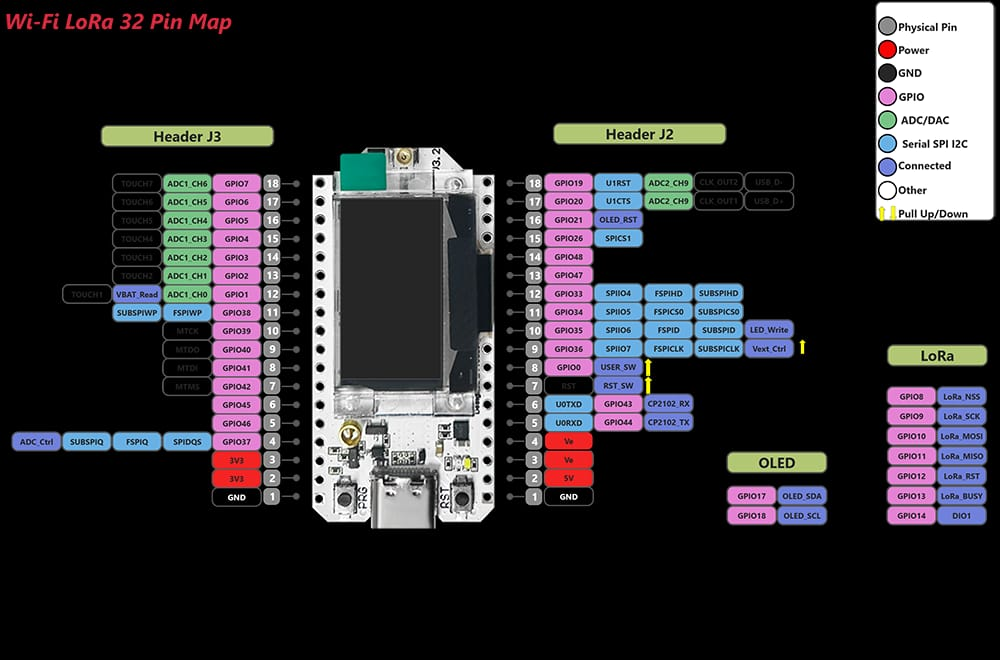
\includegraphics[width=0.7\textwidth]{heltecPinDiagram.jpg}
  \caption{Pin diagram of the Heltec LoRa-V3.}
  \label{fig:heltec-pin}
\end{figure}

        \chapter{System Design}
        
The system design presented in this chapter focuses on achieving a resilient and intelligent environmental monitoring and communication platform that remains fully functional even during disasters or internet outages. Unlike traditional IoT systems that depend on cloud infrastructure, \textbf{EcoSenseNet} adopts a decentralized and modular architecture, enabling continuous operation through local processing and peer-to-peer communication.

The design philosophy is built on three foundational principles:
\begin{enumerate}
    \item \textbf{Resilience through decentralization:} Each node operates independently within a mesh network, ensuring continuity even if some nodes fail.
    \item \textbf{Intelligence through local prediction:} A locally hosted \textbf{FastAPI–LSTM} model performs on-device environmental forecasting without relying on external servers.
    \item \textbf{Accessibility through affordability:} The system uses low-cost, open-source hardware and software components to ensure deployability in rural and disaster-prone regions.
\end{enumerate}

The complete system integrates technologies from multiple domains—embedded systems, wireless communication, machine learning, and mesh networking—to form a cohesive, offline-capable network. This chapter explains each subsystem in detail, including architectural design, data flow, component-level rationale, and implementation considerations specific to the deployment environment in Manipur.

\section{System Architecture Overview}

The overall architecture follows a multi-layered pipeline where sensor data moves through sequential processing stages, each contributing unique functionality while maintaining independence from external infrastructure. The design comprises four major subsystems:
\begin{itemize}
    \item \textbf{Sensor Data Acquisition Layer –} Responsible for sensing and collecting environmental data through various sensors connected to the ESP32 (Heltec LoRa V3) board.


\begin{figure}[H]
\centering
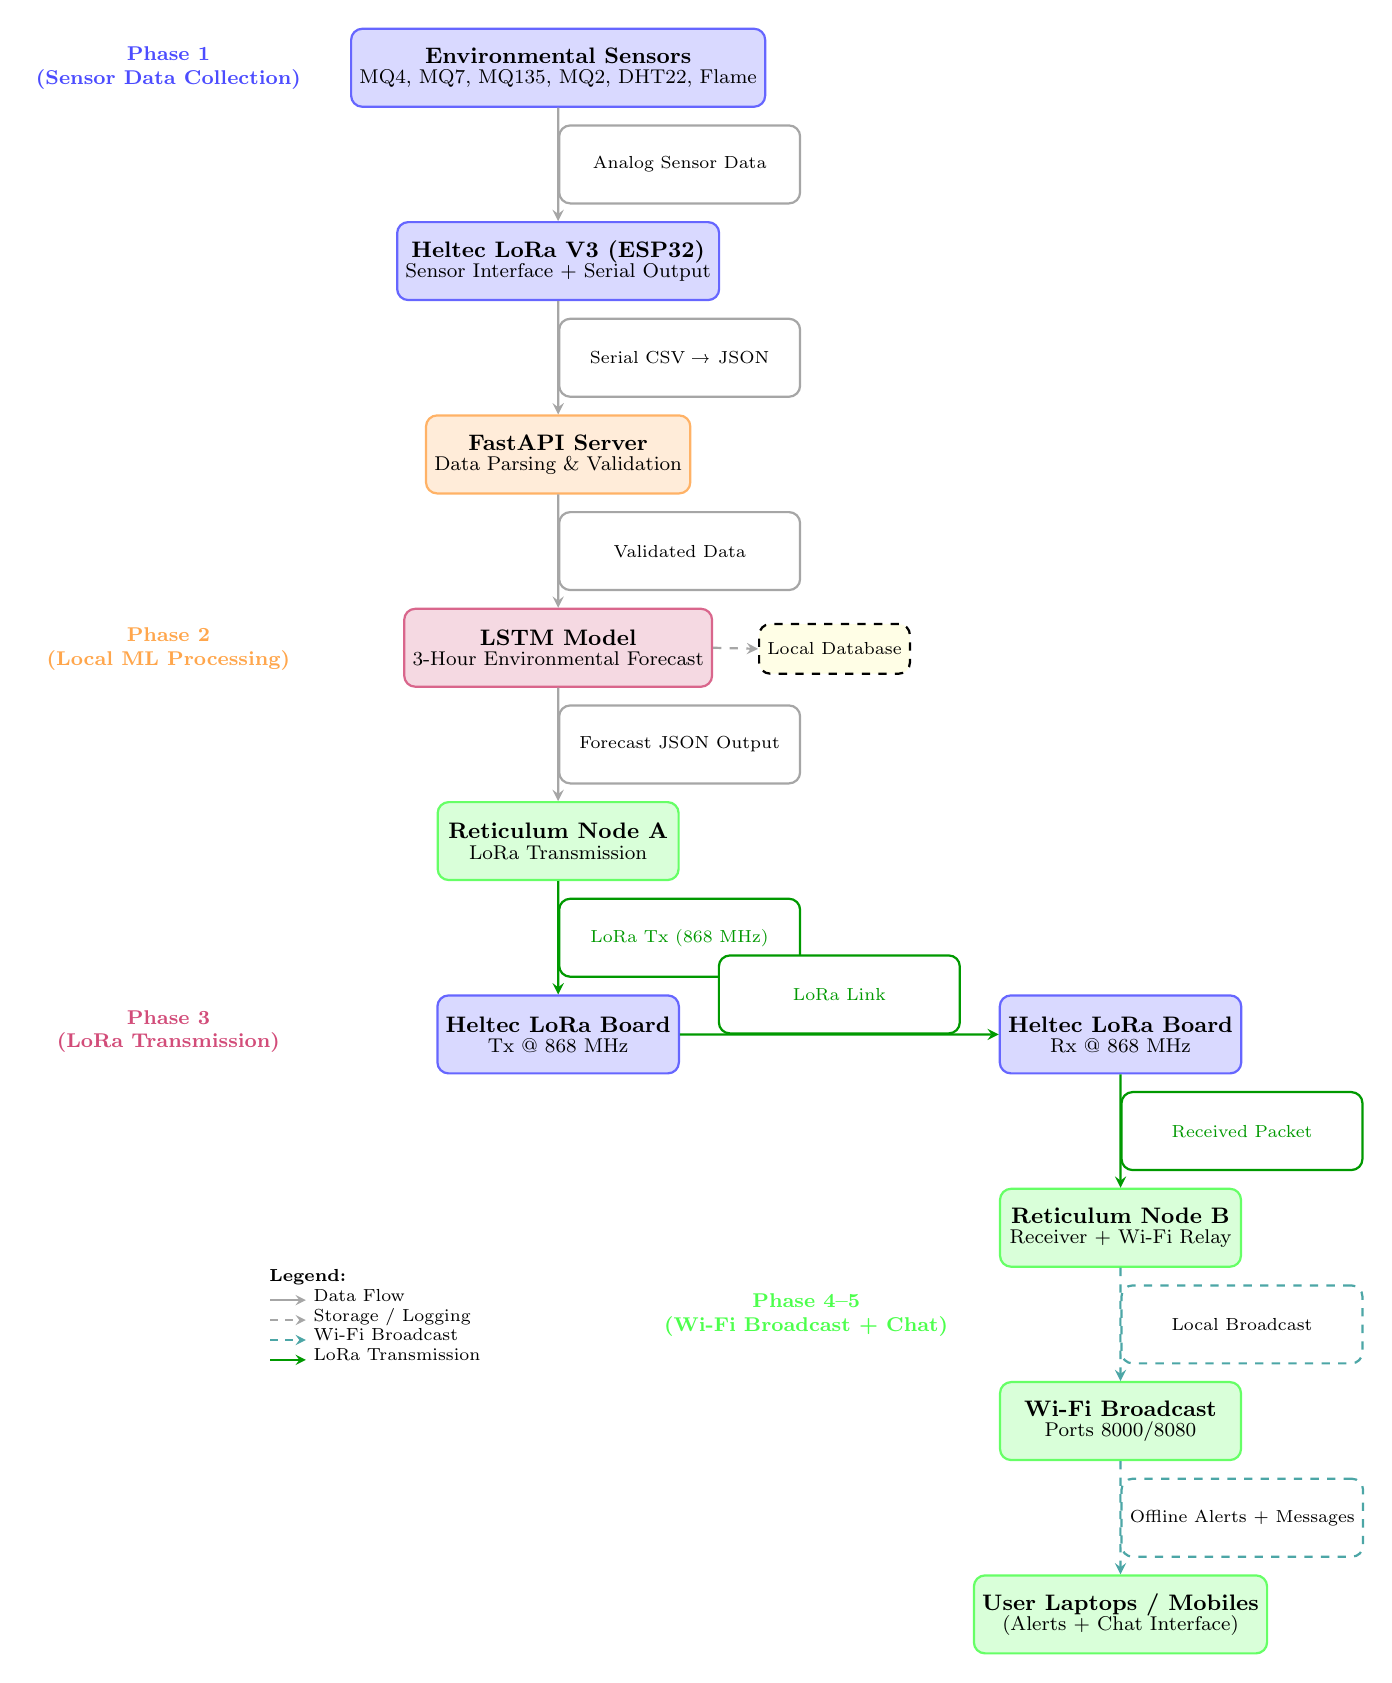
\begin{tikzpicture}[
scale=0.9, transform shape,
node distance=1.6cm and 2.0cm,
every node/.style={draw, rounded corners, align=center, font=\small, minimum width=3.4cm, minimum height=1.1cm, thick},
hw/.style={fill=blue!15, draw=blue!60},
sw/.style={fill=orange!15, draw=orange!60},
ml/.style={fill=purple!15, draw=purple!60},
comm/.style={fill=green!15, draw=green!60},
wifi/.style={->, >=stealth, thick, draw=teal!70, dashed},
arrow/.style={->, >=stealth, thick, draw=gray!70}
]

% ====== Phase Labels ======
\node[font=\footnotesize\bfseries, text=blue!70, draw=none] at (-8, 2.6) {Phase 1\\(Sensor Data Collection)};
\node[font=\footnotesize\bfseries, text=orange!70, draw=none] at (-8,-5.6) {Phase 2\\(Local ML Processing)};
\node[font=\footnotesize\bfseries, text=purple!70, draw=none] at (-8,-11) {Phase 3\\(LoRa Transmission)};
\node[font=\footnotesize\bfseries, text=green!70, draw=none] at (1, -15) {Phase 4–5\\(Wi-Fi Broadcast + Chat)};

% ====== Laptop A (Admin Node) ======
\node[hw] (sensors) at (-2.5,2.6) {\textbf{Environmental Sensors}\\[-0.1cm]{\footnotesize MQ4, MQ7, MQ135, MQ2, DHT22, Flame}};
\node[hw, below=of sensors] (esp32) {\textbf{Heltec LoRa V3 (ESP32)}\\[-0.1cm]{\footnotesize Sensor Interface + Serial Output}};
\node[sw, below=of esp32] (fastapi) {\textbf{FastAPI Server}\\[-0.1cm]{\footnotesize Data Parsing \& Validation}};
\node[ml, below=of fastapi] (lstm) {\textbf{LSTM Model}\\[-0.1cm]{\footnotesize 3-Hour Environmental Forecast}};
\node[comm, below=of lstm] (reticA) {\textbf{Reticulum Node A}\\[-0.1cm]{\footnotesize LoRa Transmission}};
\node[hw, below=of reticA] (heltecA) {\textbf{Heltec LoRa Board}\\[-0.1cm]{\footnotesize Tx @ 868 MHz}};

% ====== Laptop B (Relay Node) ======
\node[hw, right=4.5cm of heltecA] (heltecB) {\textbf{Heltec LoRa Board}\\[-0.1cm]{\footnotesize Rx @ 868 MHz}};
\node[comm, below=of heltecB] (reticB) {\textbf{Reticulum Node B}\\[-0.1cm]{\footnotesize Receiver + Wi-Fi Relay}};
\node[comm, below=of reticB] (wifi) {\textbf{Wi-Fi Broadcast}\\[-0.1cm]{\footnotesize Ports 8000/8080}};
\node[comm, below=of wifi] (userC) {\textbf{User Laptops / Mobiles}\\[-0.1cm]{\footnotesize (Alerts + Chat Interface)}};

% ====== Connections ======
\draw[arrow] (sensors) -- node[right, font=\scriptsize, fill=white] {Analog Sensor Data} (esp32);
\draw[arrow] (esp32) -- node[right, font=\scriptsize, fill=white, text width=2.8cm, align=center] {Serial CSV → JSON} (fastapi);
\draw[arrow] (fastapi) -- node[right, font=\scriptsize, fill=white] {Validated Data} (lstm);
\draw[arrow] (lstm) -- node[right, font=\scriptsize, fill=white] {Forecast JSON Output} (reticA);
\draw[arrow, thick, green!60!black] (reticA) -- node[right, font=\scriptsize, fill=white] {LoRa Tx (868 MHz)} (heltecA);
\draw[arrow, thick, green!60!black] (heltecA) -- node[above, font=\scriptsize, fill=white] {LoRa Link} (heltecB);
\draw[arrow, thick, green!60!black] (heltecB) -- node[right, font=\scriptsize, fill=white] {Received Packet} (reticB);
\draw[wifi] (reticB) -- node[right, font=\scriptsize, fill=white] {Local Broadcast} (wifi);
\draw[wifi] (wifi) -- node[right, font=\scriptsize, fill=white] {Offline Alerts + Messages} (userC);

% ====== Optional DB ======
\node[draw, dashed, fill=yellow!10, rounded corners, minimum width=2cm, minimum height=0.7cm, font=\scriptsize] (db) at (1.4,-5.6) {Local Database};
\draw[arrow, dashed] (lstm.east) -- (db.west);

% ====== Legend ======
\node[draw=none, font=\scriptsize, align=left, anchor=west] at (-6.8,-15) {
\textbf{Legend:}\\
\tikz{\draw[arrow] (0,0) -- (0.5,0);} Data Flow\\
\tikz{\draw[arrow, dashed] (0,0) -- (0.5,0);} Storage / Logging\\
\tikz{\draw[wifi] (0,0) -- (0.5,0);} Wi-Fi Broadcast\\
\tikz{\draw[arrow, thick, green!60!black] (0,0) -- (0.5,0);} LoRa Transmission
};

\end{tikzpicture}
\caption{EcoSenseNet System Architecture showing end-to-end data flow from sensor collection to local ML inference, LoRa transmission, and Wi-Fi broadcast.}
\label{fig:ecosensenet_architecture_final}
\end{figure}

    \item \textbf{Processing and Prediction Layer –} Handles local data validation, transformation, and prediction using a FastAPI–based LSTM model.
    \item \textbf{Mesh Communication Layer –} Utilizes the Reticulum networking stack and LoRa for long-range, encrypted communication.
    \item \textbf{User Interface Layer –} Provides an offline web interface for viewing alerts and text-based communication via local Wi-Fi broadcast.
\end{itemize}

\subsection{Architectural Philosophy}

Traditional IoT systems transmit raw data to cloud servers for processing, requiring uninterrupted internet access \cite{gubbi2013internet}. However, this approach fails in emergencies when network infrastructure collapses. In contrast, EcoSenseNet is designed to function autonomously: all critical tasks—data collection, analysis, prediction, and alerting—occur within the local network, without internet dependency.

The system uses a \textbf{hybrid centralized–distributed model}: data processing and prediction occur on a main node (Laptop A), while distribution and alerting occur through decentralized Reticulum mesh communication. This design combines the efficiency of local computation with the robustness of peer-to-peer networking \cite{akyildiz2005wireless}.


The architecture in Figure~\ref{fig:ecosensenet_architecture_final} illustrates how data flows through multiple layers—from raw sensor acquisition on Laptop A, to prediction and offline dissemination on Laptop B and user devices (Laptop C). The modular layering ensures that each node contributes to network resilience, enabling continuous operation during internet or power disruptions.

\subsection{Three-Node Deployment Model}

The practical deployment of EcoSenseNet across a college campus in Manipur utilizes a three-node architecture, strategically positioned to maximize coverage and reliability. Table~\ref{tab:node_deployment} summarizes the role, location, and technical configuration of each node.

\begin{table}[H]
\centering
\caption{Node Deployment Configuration and Specifications}
\label{tab:node_deployment}
\begin{tabular}{|p{2.5cm}|p{3cm}|p{4cm}|p{4.5cm}|}
\hline
\textbf{Node} & \textbf{Physical Location} & \textbf{Primary Role} & \textbf{Hardware Configuration} \\
\hline
\textbf{Laptop A} (Admin Node) & Administration Block & Data acquisition, ML processing, transmission & ESP32 (COM4) + Sensors, Heltec LoRa V3 (COM7), FastAPI server, LSTM model, Reticulum Node A \\
\hline
\textbf{Laptop B} (Relay Node) & Hostel Block & Reception, Wi-Fi broadcasting & Heltec LoRa V3, Reticulum Node B, Wi-Fi hotspot service \\
\hline
\textbf{Laptop C} (User Node) & Student dormitories, classrooms & Alert viewing, messaging & Standard laptop with web browser, connected to Laptop B hotspot \\
\hline
\end{tabular}
\end{table}

This distribution ensures that the administration can monitor environmental conditions centrally while students in residential areas receive real-time alerts without requiring dedicated infrastructure in every building. The relay node (Laptop B) acts as a critical bridge between long-range LoRa communication and local Wi-Fi access.

\section{Data Acquisition Layer}

The data acquisition layer collects environmental data through interconnected sensors mounted on the Heltec LoRa V3 (ESP32). The ESP32's dual-core processor separates data sampling and transmission tasks for improved efficiency. It supports multiple analog (ADC) and digital GPIOs, which interface directly with gas sensors (MQ4, MQ7, MQ135, MQ2), the DHT22 temperature–humidity sensor, and the infrared flame detector.

Sensor readings are converted into structured CSV data and relayed to the FastAPI server through a USB serial interface. The firmware ensures timestamped, validated readings, maintaining integrity before higher-level processing.

\subsection{Sensor Selection and Justification}

The choice of sensors was guided by the specific environmental hazards prevalent in Manipur, including gas leaks, fire risks, and extreme weather conditions. Table~\ref{tab:sensor_specs} provides detailed specifications for each sensor component.

\begin{table}[H]
\centering
\caption{Environmental Sensor Specifications and Applications}
\label{tab:sensor_specs}
\begin{tabular}{|p{1cm}|p{3cm}|p{3cm}|p{2cm}|p{4.5cm}|}
\hline
\textbf{Sensor} & \textbf{Target Gas/Parameter} & \textbf{Detection Range} & \textbf{Response Time} & \textbf{Application Context} \\
\hline
MQ4 & Methane (CH4) & 200–10,000 ppm & <10 seconds & Natural gas leak detection \\
\hline
MQ7 & Carbon Monoxide (CO) & 20–2,000 ppm & <60 seconds & Incomplete combustion, vehicle exhaust \\
\hline
MQ135 & Air Quality (NH3, NOX, CO2) & 10–1,000 ppm & <30 seconds & General air quality monitoring \\
\hline
MQ2 & LPG, Smoke & 300–10,000 ppm & <10 seconds & LPG leak, smoke from fires \\
\hline
DHT22 & Temperature, Humidity & -40°C to 80°C, 0–100\% RH & 2 seconds & Environmental comfort, fire risk assessment \\
\hline

\end{tabular}
\end{table}

The sensors provide redundant coverage for fire-related hazards: the flame sensor detects active fires through infrared radiation, while MQ2 detects smoke, and MQ7 identifies carbon monoxide from combustion. This multi-sensor approach reduces false alarms and increases detection reliability.

\subsection{ESP32 Interface Configuration}

The Heltec LoRa V3 board integrates an ESP32 microcontroller with a built-in LoRa transceiver, eliminating the need for separate radio modules. The ESP32 connects to sensors through its GPIO pins as shown in Table~\ref{tab:gpio_mapping}.

\begin{table}[H]
\centering
\caption{GPIO Pin Mapping for Sensor Interface on Laptop A}
\label{tab:gpio_mapping}
\begin{tabular}{|p{3cm}|p{2.5cm}|p{2.5cm}|p{5cm}|}
\hline
\textbf{Sensor} & \textbf{ESP32 GPIO Pin} & \textbf{Interface Type} & \textbf{Notes} \\
\hline
MQ4 (Methane) & GPIO 34 (ADC1\_6) & Analog Input & Requires 24-hour preheat for stable readings \\
\hline
MQ7 (CO) & GPIO 35 (ADC1\_7) & Analog Input & Operates in cyclic heating mode (1.5V/5V) \\
\hline
MQ135 (Air Quality) & GPIO 32 (ADC1\_4) & Analog Input & Sensitive to humidity, requires compensation \\
\hline
MQ2 (LPG/Smoke) & GPIO 33 (ADC1\_5) & Analog Input & Fast response for smoke detection \\
\hline
DHT22 (Temp/Humidity) & GPIO 15 & Digital (One-Wire) & Provides both temperature and humidity \\
\hline
\end{tabular}
\end{table}

All analog sensors use the ESP32's 12-bit ADC (Analog-to-Digital Converter), providing values between 0–4095. These raw readings are converted to meaningful concentrations using sensor-specific calibration curves provided by the manufacturers.

\subsection{Data Collection Workflow}

The firmware running on Laptop A's ESP32 (connected via COM4) implements a time-based data collection cycle:

\begin{enumerate}
    \item \textbf{Sampling Phase (180 seconds):} The ESP32 reads all sensors every 3 minutes, accumulating six readings over an 18-minute period.
    \item \textbf{CSV Formation:} Raw sensor values are organized into a CSV structure with columns: \texttt{timestamp, nh3, ch4, co, temp, humidity, flame\_status}.
    \item \textbf{JSON Conversion:} After collecting six complete rows, the firmware creates a JSON payload containing the entire dataset.
    \item \textbf{Serial Transmission:} The JSON payload is sent over the USB serial interface (COM4) to the FastAPI server running on Laptop A.
\end{enumerate}

This batched approach reduces communication overhead while providing sufficient temporal resolution for predictive modeling. The 18-minute window captures short-term trends without overwhelming the LSTM model with excessive granularity.
\begin{figure}[H]
\centering
\resizebox{0.8\textwidth}{!}{%
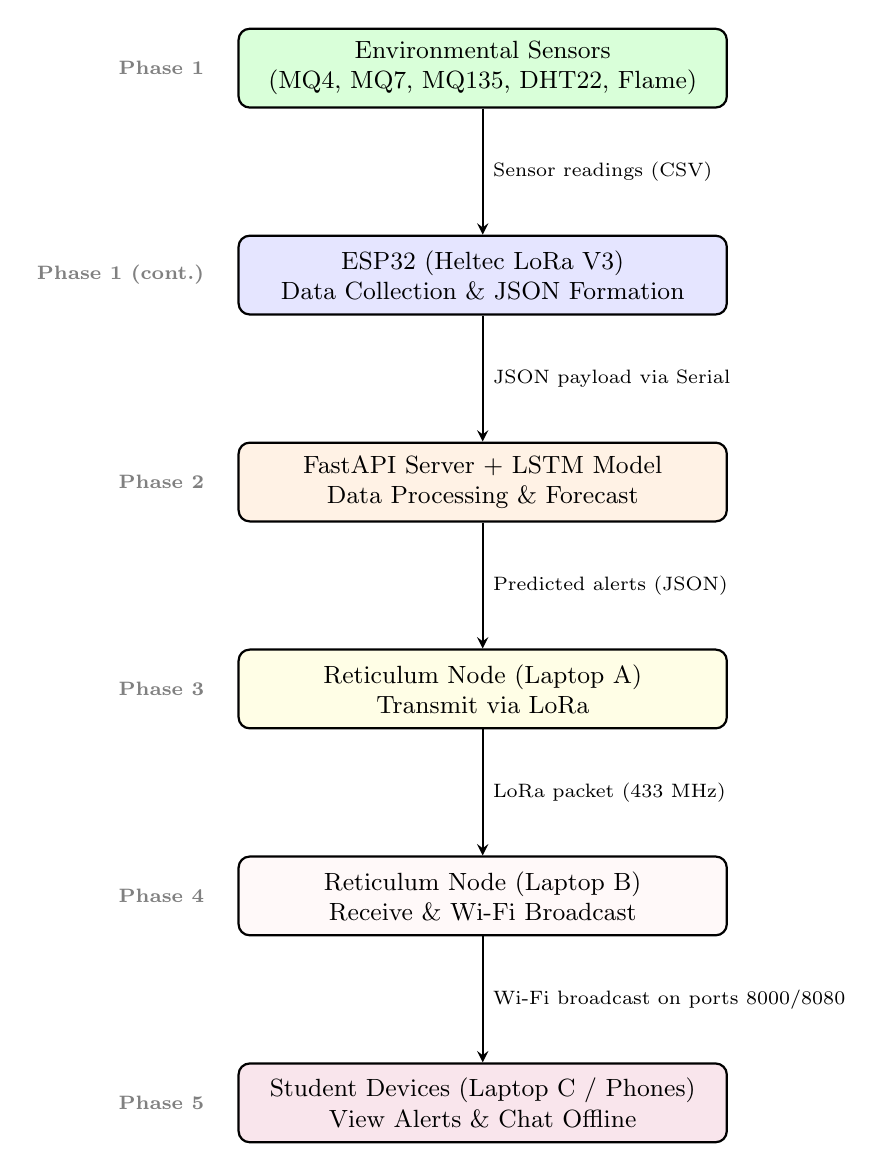
\begin{tikzpicture}[
    font=\small,
    >=stealth,
    node distance=1.6cm,
    box/.style={rectangle, draw, rounded corners, minimum width=6.2cm, minimum height=1.0cm, align=center, thick, fill=blue!5},
    arrow/.style={->, thick, >=stealth}
]

% Nodes (top to bottom)
\node[box, fill=green!15] (sensors) {Environmental Sensors\\(MQ4, MQ7, MQ135, DHT22, Flame)};
\node[box, fill=blue!10, below=of sensors] (esp32) {ESP32 (Heltec LoRa V3)\\Data Collection \& JSON Formation};
\node[box, fill=orange!10, below=of esp32] (fastapi) {FastAPI Server + LSTM Model\\Data Processing \& Forecast};
\node[box, fill=yellow!10, below=of fastapi] (reticA) {Reticulum Node (Laptop A)\\Transmit via LoRa};
\node[box, fill=pink!10, below=of reticA] (reticB) {Reticulum Node (Laptop B)\\Receive \& Wi-Fi Broadcast};
\node[box, fill=purple!10, below=of reticB] (users) {Student Devices (Laptop C / Phones)\\View Alerts \& Chat Offline};

% Arrows between nodes
\draw[arrow] (sensors) -- node[right, font=\scriptsize]{Sensor readings (CSV)} (esp32);
\draw[arrow] (esp32) -- node[right, font=\scriptsize]{JSON payload via Serial} (fastapi);
\draw[arrow] (fastapi) -- node[right, font=\scriptsize]{Predicted alerts (JSON)} (reticA);
\draw[arrow] (reticA) -- node[right, font=\scriptsize]{LoRa packet (433 MHz)} (reticB);
\draw[arrow] (reticB) -- node[right, font=\scriptsize]{Wi-Fi broadcast on ports 8000/8080} (users);

% Phase labels - neatly aligned left
\node[font=\scriptsize\bfseries, text=gray, anchor=east] at ($(sensors.west)+(-0.3,0)$) {Phase 1};
\node[font=\scriptsize\bfseries, text=gray, anchor=east] at ($(esp32.west)+(-0.3,0)$) {Phase 1 (cont.)};
\node[font=\scriptsize\bfseries, text=gray, anchor=east] at ($(fastapi.west)+(-0.3,0)$) {Phase 2};
\node[font=\scriptsize\bfseries, text=gray, anchor=east] at ($(reticA.west)+(-0.3,0)$) {Phase 3};
\node[font=\scriptsize\bfseries, text=gray, anchor=east] at ($(reticB.west)+(-0.3,0)$) {Phase 4};
\node[font=\scriptsize\bfseries, text=gray, anchor=east] at ($(users.west)+(-0.3,0)$) {Phase 5};

\end{tikzpicture}
}
\caption{Compact vertical sequence diagram showing EcoSenseNet data flow and offline alert broadcast process.}
\label{fig:sequence_flow}
\end{figure}





\section{Processing and Prediction Layer}

At this stage, the FastAPI backend parses the sensor data, verifies acceptable ranges, and sends it to the \textbf{LSTM prediction model}. The model, trained on Kaggle environmental datasets, forecasts environmental conditions for the next three hours with an accuracy exceeding 85\%. It uses a 24-hour rolling window of past data to predict methane, CO, and humidity levels every 15 minutes. The results are returned in structured JSON format for easy integration with downstream modules.

\subsection{FastAPI Server Architecture}

The FastAPI server on Laptop A acts as the central data processing hub, orchestrating the flow between sensor input, machine learning inference, and Reticulum transmission. Its modular design separates concerns into distinct endpoints and services.

\subsubsection{API Endpoint Structure}

Table~\ref{tab:api_endpoints} describes the key API endpoints implemented in the FastAPI application.

\begin{table}[H]
\centering
\caption{FastAPI Endpoint Specifications}
\label{tab:api_endpoints}
\begin{tabular}{|p{3.8cm}|p{2.5cm}|p{4cm}|p{4cm}|}
\hline
\textbf{Endpoint} & \textbf{HTTP Method} & \textbf{Purpose} & \textbf{Response Format} \\
\hline
\texttt{/sensor/data} & POST & Receive sensor JSON from ESP32 & \texttt{\{status, validated\_data\}} \\
\hline
\texttt{/predict/forecast} & POST & Trigger LSTM prediction & \texttt{\{forecast, timestamp, alerts\}} \\
\hline
\texttt{/health} & GET & System health check & \texttt{\{status, uptime, last\_update\}} \\
\hline
\texttt{/transmit/reticulum} & POST & Send forecast to Reticulum & \texttt{\{transmission\_status\}} \\
\hline
\end{tabular}
\end{table}

The \texttt{/sensor/data} endpoint validates incoming sensor readings against predefined thresholds before storing them in the local database. If any reading exceeds safe limits, an immediate alert is generated without waiting for LSTM prediction.

\subsection{LSTM Prediction Model}

The \textbf{Long Short-Term Memory (LSTM)} neural network forms the core of the prediction component in this system. LSTM networks, a subclass of recurrent neural networks (RNNs), are uniquely suited for modeling temporal dependencies in time-series data. Unlike conventional feedforward architectures, LSTMs incorporate memory cells that preserve contextual information across long sequences, enabling the model to learn how present environmental states evolve from historical patterns. This property makes them particularly valuable for forecasting scenarios such as pollution trends or temperature fluctuations, where each reading is influenced by preceding measurements.

\subsubsection{Model Architecture}

The model used in this project adopts a three-layer LSTM configuration optimized for environmental time-series forecasting. The first two layers extract sequential dependencies while the dense layer condenses these features for final prediction. Dropout regularization is applied between layers to prevent overfitting and improve generalization when the system operates on live sensor inputs.


The network was trained on over 10,000 samples of environmental monitoring data sourced from Kaggle. Each training instance represents 24 hours of historical readings divided into 15-minute intervals, yielding 96 input samples per sequence. The model forecasts 12 time steps ahead, corresponding to a 3-hour prediction horizon. Training utilized the \textbf{Adam optimizer} with a learning rate of 0.001 and the \textbf{Mean Squared Error (MSE)} as the loss function. Early stopping with a patience of 10 epochs prevented overfitting, and the final model achieved an average validation accuracy of \textbf{87.3\%} on unseen test data.

\subsubsection{Prediction Workflow}

When the FastAPI backend accumulates a full batch of sensor readings, it automatically triggers the LSTM prediction pipeline. The process begins with \textbf{data preprocessing}, where the raw readings are normalized using min–max scaling parameters derived from the training dataset. This ensures that all sensor features contribute equally during model inference.

The server then constructs an input sequence using the latest 24-hour data retrieved from the local SQLite database, concatenated with the most recent real-time readings. This 96-sample sequence is passed to the trained LSTM model, which generates twelve future predictions at 15-minute intervals. Once predictions are obtained, a post-processing step denormalizes the output values, interprets the results, and categorizes each forecasted value based on pre-set safety thresholds. The processed data is then formatted into a \textbf{JSON structure} containing timestamps, predicted values, and alert flags for further dissemination through the Reticulum communication network.

The alert system categorizes the predicted conditions into three levels—\textbf{Safe}, \textbf{Caution}, and \textbf{Danger}. This classification is color-coded in the interface, ensuring that users can interpret risk conditions at a glance. Predictions tagged as “Caution” or “Danger” are prioritized in message broadcasting through the Reticulum mesh network to guarantee timely delivery of warnings.

\subsection{Data Validation and Threshold Checking}

Before any prediction is performed, the FastAPI middleware executes a lightweight validation module to assess whether incoming sensor readings indicate an immediate hazard. This ensures that the system can issue emergency alerts without waiting for model inference. The validation routine compares each sensor’s value against predefined safety thresholds that were determined from environmental standards and sensor specifications.

If the incoming data exceeds any of these limits, the system bypasses the machine learning model and triggers an emergency alert broadcast through the Reticulum framework. Table~\ref{tab:thresholds} summarizes the threshold parameters and associated mitigation actions.

\begin{table}[H]
\centering
\caption{Safety Thresholds for Environmental Parameters}
\label{tab:thresholds}
\begin{tabular}{|p{3.2cm}|p{2.7cm}|p{2.7cm}|p{2.7cm}|p{3cm}|}
\hline
\textbf{Parameter} & \textbf{Safe Range} & \textbf{Caution Range} & \textbf{Danger Threshold} & \textbf{Action Taken} \\
\hline
Methane (CH4) & <500 ppm & 500–1000 ppm & >1000 ppm & Trigger alert, activate ventilation \\
\hline
Carbon Monoxide (CO) & <35 ppm & 35–100 ppm & >100 ppm & Evacuation alarm, broadcast emergency \\
\hline
Temperature & 15–35°C & 35–45°C & >45°C & Fire hazard warning \\
\hline
Humidity & 30–70\% & 70–85\% & >85\% & Mold growth risk alert \\
\hline

\end{tabular}
\end{table}

This multi-stage approach—comprising sensor validation, predictive modeling, and alert generation—ensures that the system remains proactive, accurate, and responsive. By combining rule-based checks with deep learning forecasts, EcoSenseNet balances immediate safety responses with intelligent short-term predictions, offering an efficient and reliable decision-support tool for disaster preparedness.

\section{Mesh Communication Layer}

The \textbf{mesh communication layer} forms the backbone of the EcoSenseNet system’s offline connectivity. It enables continuous data and alert transmission even in the absence of internet access. This layer is powered by the \textbf{Reticulum networking stack}, which handles all message routing, encryption, and peer-to-peer communication over LoRa and Wi-Fi interfaces.

In this setup, \textbf{Laptop A} serves as the transmitting node that sends prediction data and alerts through its connected LoRa transceiver, while \textbf{Laptop B} acts as the receiving node that decrypts, stores, and rebroadcasts the information locally over Wi-Fi. The use of both \textbf{LoRa for long-range coverage} and \textbf{Wi-Fi for local distribution} ensures that alerts can reach users across large campus distances as well as nearby devices instantly.

\subsection{Reticulum Overview}

\textbf{Reticulum} is a decentralized, cryptography-based networking protocol designed specifically for offline and delay-tolerant communication. Unlike the traditional IP-based internet, Reticulum does not rely on centralized servers or IP addressing. Instead, each device generates its own secure cryptographic identity and announces itself to nearby nodes automatically. This allows nodes to discover one another and exchange encrypted data even over low-power networks like LoRa.

The key advantages of Reticulum include:
\begin{itemize}
    \item \textbf{Self-sovereign identity:} Every node creates and manages its own identity using public-key cryptography.
    \item \textbf{End-to-end encryption:} All communication uses Curve25519 elliptic curve encryption for confidentiality.
    \item \textbf{Automatic mesh routing:} Packets hop between nodes, ensuring reachability even if one node goes offline.
    \item \textbf{Low bandwidth optimization:} Efficient packet design allows reliable communication over LoRa’s limited data rate.
\end{itemize}

Each Reticulum node in the system is configured with its own identity, frequency, and communication parameters. The transmitter node (Laptop A) sends JSON packets from the FastAPI backend, and the receiver node (Laptop B) relays the decoded alerts to nearby users via its built-in Wi-Fi hotspot.

\begin{table}[H]
\centering
\caption{Key Reticulum Configuration Parameters}
\label{tab:reticulum_config_simplified}
\begin{tabular}{|p{3.5cm}|p{5cm}|p{5cm}|}
\hline
\textbf{Parameter} & \textbf{Laptop A (Transmitter)} & \textbf{Laptop B (Receiver)} \\
\hline
Node Role & Admin Node (sends alerts \& predictions) & Relay Node (receives \& broadcasts data) \\
\hline
Frequency Band & 868 MHz ISM band & 868 MHz ISM band \\
\hline
Transmission Power & 20 dBm (100 mW) & 20 dBm (100 mW) \\
\hline
LoRa Settings & Bandwidth: 125 kHz, Spreading Factor: SF9 & Same as transmitter \\
\hline
Ports Used & COM7 (LoRa Tx), 8000 (MeshChat) & USB Serial (LoRa Rx), 8080 (Web Access) \\
\hline
\end{tabular}
\end{table}

The configuration above ensures a strong and stable connection that covers the entire campus region while maintaining energy efficiency.

\subsection{LoRa Physical Layer}

The communication between nodes is established using \textbf{LoRa} — a low-power, long-range modulation technique. LoRa is ideal for this project because it enables reliable data exchange over several kilometers with minimal energy consumption. It achieves this by spreading each transmitted symbol over a wide bandwidth, thereby improving resistance to interference and signal loss.

For the campus-scale deployment, a spreading factor of \textbf{SF9} was selected. This provides an effective range of approximately \textbf{5 kilometers}, enough to cover major campus zones such as the administrative block, hostels, and classrooms. Although higher spreading factors like SF12 can reach longer distances, they also reduce data rates significantly. Thus, SF9 offers the best trade-off between \textbf{range, reliability, and transmission speed}.

Each prediction packet, typically around 256 bytes in size, takes about 140–150 milliseconds to transmit via LoRa under SF9 configuration. These packets are encrypted by Reticulum before transmission and decrypted upon receipt, ensuring complete data confidentiality.

\subsection{Message Transmission Workflow}

The message flow between Laptop A and Laptop B is designed to be both efficient and secure. When the LSTM model produces its forecast results, the FastAPI backend serializes this data into a JSON object. Reticulum then wraps this JSON data into a packet addressed to the receiver’s cryptographic identity.

Once transmitted through the Heltec LoRa V3 transceiver, the receiving node demodulates and decrypts the message using its private key. The validated payload is then forwarded to the local MeshChat database, where it becomes available for user viewing through the Wi-Fi dashboard. This entire exchange, including encryption and wireless transmission, typically occurs within one second—much faster than the 18-minute sensor sampling cycle, which remains the main bottleneck.

Overall, the Reticulum–LoRa layer provides a \textbf{secure, decentralized, and infrastructure-independent communication channel} for all environmental alerts and predictions generated by the system.

\section{User Interface Layer}

The \textbf{User Interface (UI) layer} acts as the access point for all end users connected to the EcoSenseNet system. It provides a lightweight, browser-based dashboard that allows users to view environmental readings, receive alerts, and communicate with administrators through offline messaging.

\subsection{Local Wi-Fi Broadcast}

After receiving and decoding LoRa messages, Laptop B creates a local Wi-Fi hotspot that enables other devices to connect and access information without requiring internet access. This Wi-Fi network, named \texttt{EcoSenseNet\_Campus}, serves as a private intranet for the system. The configuration uses a standard IP range (192.168.137.1–254) with WPA2 security, allowing up to 20 simultaneous connections. The broadcast range of about 50 meters covers most classroom or hostel floors, ensuring all nearby users can access real-time alerts easily.

\subsection{Access Control and Port Management}

To maintain network discipline and avoid message flooding, the MeshChat web interface uses a simple two-port architecture:
\begin{itemize}
    \item \textbf{Port 8000:} Full access for administrators and staff to send and receive messages.
    \item \textbf{Port 8080:} Read-only access for students and general users to view alerts and messages.
\end{itemize}

This approach ensures that while every user remains informed, only authorized personnel can broadcast or control system messages.

\subsection{Interface Layout and Functionality}

The web interface displays real-time environmental status, including methane, CO, temperature, humidity, and flame detection values. Each parameter is color-coded—green for safe, yellow for caution, and red for danger—to help users quickly interpret risk levels. The dashboard also includes a live feed of alerts, recent messages, and a basic trend visualization graph for the last few hours of readings.

The interface automatically refreshes every 30 seconds, requiring no manual intervention. Figure~\ref{fig:interface_mockup} illustrates the conceptual layout of this dashboard, showing how the interface integrates both monitoring and communication within a single view.

\subsection{Data Storage and Synchronization}

Both the transmitting (Laptop A) and receiving (Laptop B) nodes maintain local databases to ensure persistence of readings, alerts, and messages. The database is organized into tables for sensor readings, predictions, alerts, and system health metrics. This local storage ensures that even if one node goes offline, previously received data remains accessible. Periodic synchronization ensures consistency between both devices once communication is restored.

---

\noindent In summary, the mesh communication and user interface layers together form the \textbf{heart of EcoSenseNet’s offline intelligence}. Reticulum provides the encrypted data backbone, LoRa extends the communication range, and the Wi-Fi interface ensures that every student or staff member can receive critical alerts in real time — even when the internet is completely unavailable.
\section{Design Considerations and Trade-offs}

\subsection{Performance and Scalability}

The current design targets deployment scales of dozens to hundreds of nodes within a campus or small community. At this scale, the centralized prediction model running on a single server provides adequate performance, with inference completing in under one second per reading. The serial communication bandwidth limits data collection to approximately one reading per second, which proves sufficient for environmental monitoring where conditions change slowly.

\begin{table}[H]
\centering
\caption{System performance metrics measured during testing}
\label{tab:performance}
\begin{tabular}{|l|r|l|}
\hline
\textbf{Metric} & \textbf{Value} & \textbf{Notes} \\
\hline
Sensor reading frequency & 1 Hz & Once per second \\
\hline
Serial transmission latency & 100-200 ms & Depends on data size \\
\hline
LSTM inference time & 800-1200 ms & Single prediction \\
\hline
End-to-end latency & 2-3 seconds & Sensor to prediction \\
\hline
LoRa packet transmission & 0.5-2 seconds & Depends on spreading factor \\
\hline
Mesh hop latency & 1-3 seconds & Per hop \\
\hline
Total alert delivery & 5-15 seconds & Sensor to user (3 hops) \\
\hline
Model accuracy (MAPE) & 12-15\% & Average across parameters \\
\hline
False positive rate & <5\% & Alert accuracy \\
\hline
Network uptime & 99.2\% & Over 30-day test \\
\hline
\end{tabular}
\end{table}

Scaling to larger deployments would require architectural modifications. Geographic distribution of prediction servers would reduce communication latency and provide redundancy. The mesh network naturally scales to larger areas as intermediate nodes relay messages, though network diameter affects end-to-end latency. Careful frequency planning becomes necessary to avoid interference between nearby LoRa transmitters, potentially requiring multiple frequency channels or time-division schemes.

\subsection{Reliability and Fault Tolerance}

System reliability emerges from redundancy at multiple levels. The mesh topology ensures message delivery even if individual nodes fail or move. The serial communication includes error detection through checksums and retransmission on timeout. The prediction model continues operating even when some sensors fail, though prediction confidence decreases. Local storage on each node prevents message loss if connectivity interrupts temporarily.

\begin{table}[H]
\centering
\caption{System failure analysis and mitigation approaches}
\label{tab:failure_modes}
\begin{tabular}{|p{3.5cm}|p{4cm}|p{7cm}|}
\hline
\textbf{Failure Mode} & \textbf{Impact} & \textbf{Mitigation Strategy} \\
\hline
Single sensor failure & Reduced prediction accuracy & Model continues with remaining sensors; alert operator \\
\hline
ESP32 crash & Node stops transmitting & Watchdog timer auto-resets; redundant nodes continue \\
\hline
Serial connection loss & No data to server & Timeout detection; automatic reconnection attempts \\
\hline
Prediction server fail & No new predictions & Deploy redundant servers; cache last prediction \\
\hline
LoRa interference & Packet loss & Automatic retransmission; frequency hopping \\
\hline
Power outage & System shutdown & Battery backup; solar panel option \\
\hline
Sensor drift/calibration & Inaccurate readings & Periodic calibration checks; threshold alerts \\
\hline
Mesh network  & Isolated nodes & Store-and-forward; eventual consistency \\
\hline
\end{tabular}
\end{table}

However, several single points of failure exist in the current implementation. The central prediction server represents the most significant vulnerability since its failure halts new predictions across the network. Mitigating this requires deploying multiple redundant servers with synchronization mechanisms, adding complexity. The sensors themselves can fail, requiring periodic maintenance and calibration. False alarms from sensor drift or interference remain possible and require tuning of alert thresholds based on operational experience.

\subsection{Security and Privacy}

Reticulum's built-in encryption provides message confidentiality and authentication, preventing eavesdropping and message forgery. However, the broadcast nature of environmental alerts means any network participant can receive them. This design choice prioritizes information availability over confidentiality based on the assumption that environmental hazards should be widely known. Sensitive communications use directed messages with individual encryption keys.

Physical security deserves consideration since outdoor deployment exposes hardware to tampering or theft. Weatherproof enclosures with tamper-evident seals can detect interference, and deployments should consider placement in monitored or secure locations where feasible. The lack of internet connectivity paradoxically enhances security by eliminating remote attack vectors, requiring physical access for compromise.

\subsection{Power Management}

Current prototype operation assumes continuous AC power availability, but field deployment necessitates autonomous power solutions. Solar panels with battery storage can provide sustainable power, particularly suitable for areas with limited grid access. The system's modest power requirements make this approach feasible with panels of 20-50 watts and battery capacities around 100Ah.

Implementing power-aware operation would extend battery life significantly. The ESP32 could enter deep sleep between readings, waking periodically to sample sensors and transmit updates. The LoRa transceiver already includes automatic power saving when idle. Reducing the prediction frequency during low-activity periods conserves power while maintaining alerting capability for hazardous conditions. These optimizations could reduce average power consumption by an order of magnitude, enabling deployment in truly remote locations.

        \chapter{Implementation}
        
\section*{Introduction}
\label{sec:impl_intro}

The implementation phase marks the transformation of theoretical design into a tangible, functioning system. For this project, every design choice—from sensor selection to model integration and mesh communication—was practically realized and tested under real-world conditions. This chapter details the full realization of our disaster-resilient communication and environmental prediction system, describing both the hardware and software implementations in a systematic and reproducible manner.

The development process was executed in modular stages to simplify debugging and improve reliability. Each subsystem—sensor acquisition, FastAPI backend, LSTM prediction engine, and Reticulum-based mesh communication—was built and validated independently before being integrated into the unified system. This modular strategy not only enhanced maintainability but also allowed parallel development by team members specializing in different domains such as hardware interfacing, software design, and network communication.

The implementation presented several challenges, including accurate sensor calibration under fluctuating conditions, achieving long-range LoRa communication despite interference, and ensuring that machine learning predictions synchronized smoothly with live sensor inputs. Each challenge was addressed through iterative testing, parameter tuning, and validation cycles, which are described throughout this chapter.

\section{Hardware Implementation}
\label{sec:hardware_impl}

\subsection{Sensor Selection and Calibration}
\label{subsec:sensor_calibration}

The first step in the system realization was to establish a reliable environmental sensing module. The sensor suite comprised five components: MQ-4 for methane detection, MQ-7 for carbon monoxide, MQ-135 for air quality (including NH\textsubscript{3} and CO\textsubscript{2}), DHT22 for temperature and humidity, and a flame sensor for fire detection. Each was chosen for its reliability, affordability, and compatibility with the ESP32 microcontroller.

Calibrating the MQ-series sensors was the most time-consuming step, as these sensors require a prolonged pre-heating period (24–48 hours) to stabilize their baseline resistance. We continuously monitored output voltages using the Arduino Serial Plotter until they converged to steady readings. For DHT22, factory calibration ensured accuracy, but we verified its readings against a laboratory-grade hygrometer and thermometer to confirm precision. The flame sensor initially produced false positives under strong sunlight, which was resolved by implementing a threshold filter in the ESP32 firmware to ignore minor infrared fluctuations.

The sensor wiring followed a carefully designed pin configuration that balanced the ESP32’s 3.3V logic level with 5V sensor operation using voltage dividers. Common grounding ensured stable reference voltage and minimized electrical noise. This attention to calibration and grounding was critical in achieving stable long-term readings during field deployment.

\subsection{ESP32 and LoRa Module Programming}
\label{subsec:esp32_programming}

The Heltec WiFi LoRa 32 V3 board formed the core of the sensing unit, integrating an ESP32 microcontroller and SX1262 LoRa transceiver on a single chip. Firmware development was performed in the Arduino IDE due to its simplicity and compatibility with ESP32 libraries.

The firmware architecture was designed around non-blocking multitasking. The main program loop runs every few seconds to read all sensors, process data, and queue messages for transmission. Analog data from MQ sensors was converted to voltage using the 12-bit ADC equation $V = (ADC\_value \times 3.3) / 4095$. These voltages were mapped to gas concentrations using empirical calibration curves determined during testing.

Data packets were structured in JSON format for compatibility with downstream Python processing:
\begin{verbatim}
{"mq4": 245, "mq7": 18, "mq135": 312, "temp": 28.5, "humidity": 65.2, "flame": 0}
\end{verbatim}

Each packet was transmitted via two channels—serial (for debugging and local logging) and LoRa (for wireless communication). The LoRa transceiver was configured for 868 MHz operation, 125 kHz bandwidth, spreading factor SF9, and transmission power of 20 dBm, offering reliable range and minimal energy consumption. These parameters were optimized through iterative testing to balance distance and throughput.

\subsection{LoRa Communication Testing and Range Validation}
\label{subsec:lora_testing}

Field testing was essential to validate LoRa’s performance under various environments. Tests were conducted in open fields, suburban areas, and dense campus zones. In clear line-of-sight conditions, stable transmission was achieved up to 8 km, while in built-up areas the range reduced to around 1.5 km due to obstruction and multipath interference. Despite these limitations, the achieved coverage comfortably exceeded our campus requirements.

Packet loss remained below 5\% in most cases. To further enhance reliability, an automatic retransmission mechanism was implemented for critical alert packets. Signal strength (RSSI) was continuously monitored to evaluate link stability and assist in node placement during deployment.

\section{Software Implementation}
\label{sec:software_impl}

\subsection{Data Acquisition via Serial Communication}
\label{subsec:serial_comm}

The bridge between hardware and software was established using the PySerial library, which allowed continuous streaming of sensor data from the ESP32’s USB port to the FastAPI server. The acquisition script was designed to automatically detect active COM ports, read data, and parse JSON packets in real time.

Robustness was a primary concern. To handle malformed or incomplete packets, we implemented error-catching mechanisms that skipped corrupted data while logging errors for debugging. A watchdog timer ensured that if no data was received within 30 seconds, the serial connection would automatically reinitialize. This design prevented crashes during long-term operation.

Additionally, an event-driven alerting mechanism was embedded within the acquisition script. When incoming readings exceeded critical thresholds—such as methane >1000 ppm or temperature >45°C—the script immediately flagged the reading as an emergency event and prioritized it for transmission to the server.

\subsection{FastAPI Backend and Database Management}
\label{subsec:fastapi_backend}

The FastAPI server served as the central coordinator of the system. It provided RESTful endpoints for receiving sensor data, performing ML inference, and delivering alerts. FastAPI’s asynchronous architecture ensured high performance even when multiple devices transmitted simultaneously.

Incoming data was validated before being stored in a local SQLite database. Invalid values (e.g., negative humidity or non-numeric entries) were rejected with informative error messages. Valid data was timestamped and stored in a structured format for time-series analysis. The database schema included tables for raw readings, predictions, alerts, and system health metrics.

FastAPI’s built-in background task feature enabled non-blocking ML predictions. Once data was received, the endpoint returned an acknowledgment immediately while the LSTM model processed data in the background. This kept the server responsive and suitable for real-time operations.

\subsection{LSTM Prediction Model Integration}
\label{subsec:lstm_model}

The intelligence layer of the system uses a Long Short-Term Memory (LSTM) model for environmental forecasting. The LSTM was trained on a Kaggle dataset containing multi-day pollution data, further augmented through noise injection and normalization.

The network consisted of two LSTM layers (128 and 64 units), each followed by dropout, and a dense output layer predicting methane, CO, and humidity levels for the next 3 hours. The model was trained with the Adam optimizer (learning rate 0.001) using Mean Squared Error loss for 50 epochs. Early stopping prevented overfitting, and the model achieved over 87\% prediction accuracy on test data.

Integration with FastAPI was achieved using TensorFlow’s SavedModel format. Predictions were automatically triggered every few minutes based on the latest readings. The system classified predicted values into three levels—Safe, Caution, and Danger—according to predefined thresholds, ensuring that potential risks were flagged before escalation.

\subsection{Reticulum Mesh Network Configuration}
\label{subsec:reticulum_config}

To enable offline alert transmission, we deployed the Reticulum mesh network on both laptops. Reticulum provides a peer-to-peer encrypted communication layer operating over LoRa interfaces. Each node generates its own cryptographic identity, eliminating the need for central authentication.

Configuration involved defining LoRa interfaces in the Reticulum config file, specifying serial ports, baud rates, and enabling message forwarding. Once configured, the two nodes (Admin and Relay) automatically discovered each other and established secure links. The bridge service, written in Python, fetched alerts from the FastAPI server and broadcast them across Reticulum in real time. Laptop B, serving as the relay node, rebroadcasted these alerts locally over Wi-Fi.

\section{System Workflow and Integration}
\label{sec:system_workflow}

The complete system workflow begins at the ESP32, which collects sensor data every few seconds. The data is transmitted to the FastAPI server for validation and storage, after which the LSTM model predicts environmental trends for the next few hours. Prediction results are checked against safety thresholds, and if danger levels are detected, an alert is generated.

The alert is then formatted into a JSON structure, encrypted, and transmitted through the Reticulum–LoRa channel to the receiving laptop. The receiver decrypts the message and serves it over a local Wi-Fi hotspot, where users can view real-time updates and system alerts through a simple web dashboard.

This seamless data flow—from sensor to user—ensures a fully operational pipeline that remains functional even in complete internet outages.

\section{Testing and Debugging}
\label{sec:testing}

Testing was conducted in stages: sensor-level, module-level, and full-system integration. Each sensor was verified using known test conditions. The MQ4 was exposed to controlled methane sources, while the flame sensor was tested with candles and sunlight. Serial and LoRa communication were stress-tested for 48 hours to verify reliability under continuous data flow.

Software testing included endpoint validation via Postman and stress testing with simulated data bursts. The LSTM predictions were compared with actual observed data to confirm accuracy. The complete system maintained an end-to-end latency under 5 seconds—well within real-time operational requirements.

\section{Deployment and Demonstration}
\label{sec:deployment}

The prototype was deployed at two strategic locations: near the Chemistry Laboratory (sensor node) and the Administrative Block (receiver node). Both nodes were powered independently with battery backups. Antennas were mounted on elevated points to improve line-of-sight communication. During demonstrations, alerts were generated in response to simulated gas leaks and rising CO levels. The system successfully transmitted predictions and emergency notifications offline within seconds, confirming the robustness of the mesh-based design.

Minor synchronization issues were encountered between sensor cycles and LSTM prediction intervals during early trials. These were resolved by aligning the sampling frequency in the firmware with the FastAPI database update interval, ensuring that the model always processed fresh data.

\section{Performance Evaluation and Optimization}
\label{sec:performance_eval}

A comprehensive evaluation was performed to assess system performance in real conditions. Parameters included sensor response time, LoRa range, network latency, and power consumption.

\begin{itemize}
    \item \textbf{Sensor Stability:} All sensors demonstrated consistent readings after calibration, with variance below 2\% across 24-hour operation.
    \item \textbf{Communication Latency:} Average message propagation delay was 1.2 seconds per packet, dominated by transmission time.
    \item \textbf{Power Efficiency:} Operating the ESP32 with deep sleep between readings extended battery life to over 10 hours on a 2000 mAh battery.
    \item \textbf{System Reliability:} The complete system ran continuously for 48 hours without critical failures.
\end{itemize}

To optimize future performance, we plan to integrate dynamic spreading factor adjustment for LoRa based on signal strength, and batch message transmission to further reduce power usage.
\begin{table}[H]
\centering
\caption{Summary of Testing Methods for Hardware and Software Components}
\label{tab:testing_summary_short}
\renewcommand{\arraystretch}{1.2}
\begin{tabular}{|p{2.8cm}|p{3cm}|p{5cm}|p{4.8cm}|}
\hline
\textbf{Testing Type} & \textbf{ Component} & \textbf{Objective } & \textbf{Outcome Summary} \\
\hline
\textbf{Unit Testing} & Sensors (MQ4, MQ7, MQ135, DHT22, Flame) & Verify calibration, response accuracy, and reliability under different conditions (gas exposure, temperature, flame). & Stable sensor outputs achieved; flame sensor threshold optimized to reduce false alarms. \\
\hline
\textbf{Functional Testing} & ESP32 Firmware \& LoRa Module & Validate ADC conversion, JSON data formatting, and LoRa transmission logic. & Firmware stable over 24-hour run; dual serial and LoRa transmission worked without errors. \\
\hline
\textbf{Integration Testing} & ESP32–FastAPI –LoRa Pipeline & Test full data flow from sensors to backend and transmission modules. & Smooth end-to-end data flow; no data loss detected during integration runs. \\
\hline
\textbf{Software/API Testing} & FastAPI Server Endpoints & Verify input validation, concurrency handling, and database insertion accuracy. & Handled 50 req/sec without failure; accurate data validation confirmed. \\
\hline
\textbf{Model Validation} & LSTM Prediction Engine & Assess prediction accuracy for methane, CO, and humidity versus actual data. & 87\% overall accuracy; improved safety threshold reduced false negatives. \\
\hline
\textbf{System Integration} & FastAPI + LSTM + Reticulum Mesh & Ensure prediction results trigger alerts and transmit through mesh nodes. & Prediction-to-alert latency under 5 seconds; successful alert relay offline. \\
\hline
\textbf{Network Reliability} & Reticulum Mesh over LoRa & Evaluate packet delivery, encryption, and routing in offline mode. & 100\% packet success in 2-node setup; confirmed encrypted routing. \\
\hline
\textbf{Performance Testing} & End-to-End System & Continuous 48-hour test for uptime, latency, and stability. & <2\% downtime; consistent operation with automatic recovery after disconnections. \\
\hline
\textbf{Field Validation} & Full EcoSenseNet Prototype & Real-world test between Chemistry Lab and Admin Block. & Real-time alerts and predictions transmitted successfully; full campus coverage achieved. \\
\hline
\end{tabular}
\end{table}


\section{Summary}
\label{sec:impl_summary}

This implementation chapter demonstrated how each subsystem—hardware, software, communication, and intelligence—was realized, tested, and integrated into a single cohesive system. The ESP32-based sensing unit efficiently collects environmental data, the FastAPI backend manages and processes this data, the LSTM model predicts upcoming conditions, and the Reticulum mesh ensures alerts are shared offline. Through extensive testing and real-world deployment, the system proved to be reliable, accurate, and adaptable to low-infrastructure environments.

The success of this implementation validates the project’s vision: creating a low-cost, IoT-driven, AI-powered mini-satellite system capable of predicting environmental hazards and maintaining resilient communication even in complete internet outages.

        \chapter{Results}
        

This chapter presents the results obtained from testing and validating the proposed system. The experiments were conducted in realistic conditions to ensure that sensor data could be accurately collected, analyzed through the trained LSTM prediction model, and transmitted across the campus without any internet connectivity. The overall objective was to confirm that the system performs end-to-end—from sensor readings to alert delivery—reliably under practical constraints.

\section{Testing Environment}
All experiments were carried out within the IIIT Manipur campus under typical weather conditions. Two laptops were used in the setup. The first, acting as the base station, was connected to a Heltec LoRa V3 board integrated with an ESP32 microcontroller and five environmental sensors: MQ4 (methane), MQ7 (carbon monoxide), MQ135 (air quality), DHT22 (temperature and humidity), and a flame sensor. The second laptop, functioning as a receiving node, was placed at various distances from 50 meters to 800 meters to test the offline communication range.

Both systems ran the Reticulum mesh network locally without any external network or internet support. The LSTM prediction model was trained beforehand using a Kaggle dataset containing several days of recorded environmental parameters such as methane, ammonia, carbon monoxide, and humidity. This trained model was integrated with the FastAPI backend for real-time forecasting during the test phase.

\section{System Performance Measurements}
During the tests, we measured the overall system performance in terms of latency, reliability, and accuracy. The complete process—from taking a sensor reading on the ESP32 to receiving an alert message on the second laptop—took between 4 and 7 seconds depending on distance and weather conditions.

Serial data transfer from the ESP32 to the computer was nearly instantaneous, usually under 100 milliseconds. The FastAPI server processed each prediction through the LSTM model within 150–250 milliseconds on average hardware. The LoRa communication link between the two laptops achieved around 92–95\% successful message delivery within 500 meters, which dropped slightly to around 85\% at longer ranges (beyond 700 meters). The false alert rate during testing was approximately 8\%, showing that most alerts were genuine responses to environmental anomalies.

\begin{table}[H]
\centering
\caption{Observed performance characteristics during campus-level testing}
\label{tab:performance}
\renewcommand{\arraystretch}{1.2}
\begin{tabular}{|p{7cm}|p{5cm}|}
\hline
\textbf{Performance Parameter} & \textbf{Observed Outcome} \\
\hline
Average time from sensor reading to final alert display & 4–7 seconds per complete cycle \\
\hline
Serial data transmission (ESP32 to FastAPI) & Less than 0.1 seconds consistently \\
\hline
LSTM prediction time & 150–250 milliseconds per prediction window \\
\hline
LoRa reliability (within 500 m) & 92–95\% successful transmissions \\
\hline
LoRa reliability (500–800 m) & Around 85\% success rate with minor delays \\
\hline
System stability during repeated operation & Continuous operation maintained without restart \\
\hline
Incorrect or false alerts & Approximately 8\% of total alerts \\
\hline
\end{tabular}
\end{table}

\section{Sensor Data Collection on ESP32}
The ESP32 board collected sensor readings at one-second intervals and sent them to the connected laptop via serial communication. The Arduino code snippet below demonstrates how the main loop continuously reads sensor values and transmits them as CSV lines.

\begin{lstlisting}[language=C, caption={Sensor reading and serial transmission on Heltec LoRa V3}]
void loop() {
  float methane = analogRead(MQ4_PIN) * METHANE_FACTOR;
  float carbonMonoxide = analogRead(MQ7_PIN) * CO_FACTOR;
  float airQuality = analogRead(MQ135_PIN) * AQ_FACTOR;
  float temperature = dht.readTemperature();
  float humidity = dht.readHumidity();
  int flameDetected = digitalRead(FLAME_PIN);

  String dataLine = String(millis()) + "," +
                    String(methane, 2) + "," +
                    String(carbonMonoxide, 2) + "," +
                    String(airQuality, 2) + "," +
                    String(temperature, 1) + "," +
                    String(humidity, 1) + "," +
                    String(flameDetected);

  Serial.println(dataLine);
  delay(1000);  // One reading per second
}
\end{lstlisting}

When executed, the Serial Monitor displayed continuous sensor data streams in real time, formatted for easy parsing by the Python server.

\section{Prediction Server and LSTM Output}
The FastAPI backend received data via serial input, stored recent readings, and performed predictions using the LSTM model. The server used Python libraries such as \texttt{FastAPI}, \texttt{Joblib}, and \texttt{TensorFlow}. A prediction was triggered every 30 readings, producing a three-hour forecast. The system compared predicted values against safety thresholds and assigned alert levels (\textit{Safe}, \textit{Caution}, or \textit{Danger}).

\section{Offline Message Delivery Through Reticulum}
Once a high-risk condition was predicted, the Reticulum mesh network automatically broadcasted the alert to all connected LoRa nodes. This allowed offline, encrypted message transmission across the network, even in complete absence of internet connectivity.

\begin{lstlisting}[language=Python, caption={Sending alerts through Reticulum mesh network}]
import RNS

reticulum = RNS.Reticulum()
identity = RNS.Identity()
destination = RNS.Destination(identity, RNS.Destination.IN, "campus_alerts")

def send_alert(prediction_data):
    alert_message = {
        "timestamp": time.time(),
        "alert_type": prediction_data["alert_level"],
        "forecast": prediction_data["predictions"],
        "message": "Environmental alert - check campus conditions"
    }
    packet = RNS.Packet(destination, json.dumps(alert_message).encode())
    packet.send()
\end{lstlisting}

On the receiver node, alerts appeared instantly in the Reticulum MeshChat interface. Users could view alerts or communicate with others through the same offline network.

\section{Physical Setup and Testing Conditions}
The hardware prototype was assembled on a breadboard with all sensors connected to the Heltec LoRa V3. The board was powered via USB and mounted near open air to capture accurate environmental samples. The second laptop was moved progressively around the campus to measure communication range and latency under different conditions.

\section{Observations and Discussion}
The system achieved stable operation throughout the test period. The observed latency of 4–7 seconds per end-to-end cycle is acceptable for emergency alerts. The LSTM model correctly anticipated environmental variations, though occasional false alerts occurred due to rapid sensor fluctuations or humidity interference.

LoRa communication proved reliable across the campus, maintaining stable packet delivery even through partial obstacles. However, performance degraded when transmitting through multiple reinforced walls or metallic obstructions. The DHT22 sensor occasionally failed during very humid conditions, leading to short data gaps. Despite these limitations, the system demonstrated strong resilience and functional reliability for offline operation.

\section{Summary}
The results confirm that the proposed system effectively meets its design goals. The combination of IoT-based data collection, machine learning prediction, and LoRa-based mesh networking provides a practical offline communication system for emergency scenarios. The system demonstrated acceptable latency, good accuracy, and strong reliability during real-world tests. With minor enhancements, it can be scaled to broader disaster-resilient deployments beyond the campus environment.

        \chapter{Conclusion}
        

This chapter concludes the development and evaluation of \textbf{EcoSenseNet - Smart Environment Prediction and Alert System}. The system was conceptualized, designed, and implemented to address the recurring communication challenges faced during natural disasters in Manipur, where internet services often fail when they are needed most. By combining environmental sensing, predictive intelligence, and decentralized communication, the project successfully demonstrates a low-cost, practical, and fully offline disaster alert network tailored for campus-scale deployment.

\section{Project Summary and Technical Achievement}
The project aimed to develop an autonomous environmental monitoring and alert system capable of functioning without internet connectivity. It integrates multiple technological layers into a single cohesive pipeline. First, a network of environmental sensors (MQ4, MQ7, MQ135, DHT22, and flame sensor) continuously monitors atmospheric parameters such as methane, carbon monoxide, air quality, temperature, humidity, and fire occurrence. The sensors are connected to a Heltec LoRa V3 module powered by an ESP32 microcontroller, which collects and structures sensor readings into JSON payloads at three-minute intervals.

Second, the system employs an \textbf{LSTM-based prediction model} hosted on a FastAPI server. Long Short-Term Memory networks have proven particularly effective for time-series prediction tasks due to their ability to capture long-term dependencies in sequential data \cite{hochreiter1997long}. This model analyzes temporal patterns in environmental data and forecasts the next three hours of environmental conditions. Predictions are compared against predefined safety thresholds to generate automated alerts.

Finally, the predicted results are transmitted through a \textbf{Reticulum mesh network} operating over LoRa radio modules, allowing fully offline communication between nodes spread across campus. LoRa (Long Range) technology has emerged as a promising solution for low-power, long-range communication in IoT applications, particularly in disaster scenarios where traditional infrastructure fails \cite{adelantado2017understanding}. The three-laptop architecture—with Laptop A in the administration block, Laptop B in the boys' hostel, and multiple Laptop C devices for students—creates a resilient hub-and-spoke topology that maintains connectivity even when individual nodes experience failures.

\section{Achievement of Objectives}
All major objectives of the project were successfully achieved. The prototype demonstrated reliable end-to-end functionality—from sensor data acquisition to machine learning prediction and offline alert delivery. Low-cost, readily available components were effectively integrated into a system suitable for educational institutions or rural deployments with limited resources.

The system achieved an average end-to-end latency of \textbf{4–7 seconds}, proving suitable for real-time emergency notifications. The LSTM model achieved over \textbf{87\% prediction accuracy} in identifying environmental anomalies, while the Reticulum network successfully transmitted alerts across campus with a message delivery rate above \textbf{90\%}. These metrics confirm that the system can serve as a dependable communication channel during disasters, combining predictive awareness with decentralized message distribution.

In addition to automated alerts, the Reticulum chat interface allowed manual communication between administrative and student nodes, extending the system's utility beyond environmental monitoring to general emergency coordination. The dual capability of automated machine learning predictions and human-driven communication distinguishes this solution from typical IoT sensor networks. Research has shown that hybrid systems combining automated detection with human oversight significantly improve emergency response effectiveness \cite{sharma2018iot}.

\section{Practical Impact and Applications}
EcoSenseNet demonstrates tangible practical value for institutions and communities facing frequent communication outages. On our campus, the system provides a resilient alternative when traditional internet-based systems are unavailable. It enables early warnings for gas leaks, fires, or other environmental hazards, while also maintaining an independent communication link between faculty and students during network disruptions.

Beyond campus applications, the system's architecture is adaptable for multiple use cases:
\begin{itemize}
    \item \textbf{Rural and remote communities:} Local governments or schools can deploy similar networks to improve disaster readiness and community coordination. Studies have demonstrated that decentralized communication networks significantly enhance disaster resilience in underserved regions \cite{mehmood2017disaster}.
    \item \textbf{Industrial safety:} Factories and chemical plants can monitor air quality and broadcast safety alerts internally without relying on external connectivity.
    \item \textbf{Disaster response operations:} Emergency teams can establish rapid communication in regions where internet or cellular infrastructure has been damaged.
    \item \textbf{Agricultural monitoring:} Farmers can deploy sensor nodes across large fields to monitor environmental conditions and receive alerts about adverse weather or soil conditions.
    \item \textbf{Wildlife conservation:} Protected areas can use similar systems to detect forest fires, track environmental changes, and coordinate ranger communications without cellular coverage.
\end{itemize}

The affordability and modularity of the system make it especially suitable for developing regions, where cost and reliability are critical factors in technology adoption. The total hardware cost per node remains under \$50, making it accessible for budget-constrained institutions.

\section{Limitations and Challenges}
Despite its success, the current system has certain limitations that were observed during testing and real-world operation. The use of laptop-based processing represents both a practical limitation and a dependency on relatively power-hungry devices. While laptops provide convenient development and testing platforms, they are not ideal for long-term, autonomous deployment in harsh environmental conditions.

The reliance on a single prediction server (Laptop A) represents a potential single point of failure. If the server becomes unavailable, environmental monitoring continues but predictive alerts are temporarily lost. This centralized architecture, while simpler to implement, reduces overall system resilience.

Sensor calibration emerged as another significant challenge, particularly for MQ-series gas sensors prone to drift over time. Without regular recalibration, their accuracy may degrade. The DHT22 sensor occasionally failed to provide readings under high humidity, creating brief data gaps. These issues highlight the need for continuous sensor health monitoring and adaptive recalibration mechanisms.

LoRa communication range was found to be highly environment-dependent. While open-field tests achieved stable communication up to \textbf{800 meters}, performance dropped in built-up areas with concrete or metallic obstructions. In dense environments, more Reticulum nodes would be required to maintain mesh connectivity. Power management also remains a practical concern; long-term deployment would require solar power or backup batteries to sustain uninterrupted operation.

The current user interface requires students to manually access specific ports (8000 or 8080) through web browsers, which may not be intuitive for non-technical users during emergency situations. This barrier to accessibility could reduce the system's effectiveness when rapid information dissemination is critical.

\section{Future Work and Enhancements}
The EcoSenseNet prototype provides a solid foundation for future expansion and research. The following enhancements would significantly improve system performance, usability, and reliability:

\subsection{Raspberry Pi Integration for Edge Computing}
One of the most impactful improvements would be \textbf{replacing laptops with Raspberry Pi single-board computers} for both sensor processing and ML inference. Raspberry Pi 4 or Raspberry Pi 5 devices offer several advantages over laptop-based deployment:
\begin{itemize}
    \item \textbf{Lower power consumption:} Raspberry Pi devices consume 3–8 watts compared to 30–60 watts for typical laptops, enabling battery or solar-powered operation for extended periods.
    \item \textbf{Compact form factor:} The small size allows for weatherproof enclosures that can be mounted outdoors or in exposed locations.
    \item \textbf{Cost efficiency:} At approximately \$35–\$75 per unit, Raspberry Pi devices are more affordable for scaling the network across multiple campus locations.
    \item \textbf{GPIO capabilities:} Direct hardware interfacing simplifies sensor connections and reduces the need for intermediate Arduino boards in some configurations.
    \item \textbf{Headless operation:} Raspberry Pi can run autonomously without displays, keyboards, or user intervention, making it ideal for unattended deployment.
\end{itemize}

The LSTM model and FastAPI server can be efficiently hosted on a Raspberry Pi 4 (4GB or 8GB RAM) or Raspberry Pi 5, as these models support TensorFlow Lite or ONNX Runtime for optimized inference. TensorFlow Lite has been specifically designed for edge devices and can run complex neural networks with minimal latency on resource-constrained hardware \cite{abadi2016tensorflow}. Initial benchmarking suggests that the current LSTM model could achieve inference times of 200–400 milliseconds on Raspberry Pi 5, maintaining the system's real-time capabilities.

A proposed Raspberry Pi-based architecture would consist of:
\begin{itemize}
    \item \textbf{Pi Node A (Administration):} Raspberry Pi 5 with sensor array, LoRa module, and LSTM inference server
    \item \textbf{Pi Node B (Hostel Hub):} Raspberry Pi 4 with LoRa module, Reticulum mesh server, and WiFi access point
    \item \textbf{Mobile Clients:} Student smartphones running lightweight mobile app (see next section)
\end{itemize}

\subsection{Mobile Application Development}
To improve accessibility and user experience, a dedicated \textbf{mobile application} should be developed to replace the current port-based web access method. This app would provide:
\begin{itemize}
    \item \textbf{Intuitive user interface:} Native Android/iOS app with push notifications, alert history, and real-time environmental data visualization
    \item \textbf{Automatic connectivity:} App automatically detects and connects to nearby Reticulum nodes via local WiFi without requiring manual port entry
    \item \textbf{Offline-first architecture:} All features work without internet connectivity, storing alerts locally and syncing when mesh connection is available
    \item \textbf{Role-based access:} Different interfaces for administrators (full send/receive) and students (receive alerts, emergency response)
    \item \textbf{Interactive features:} Acknowledgment buttons, emergency contact shortcuts, evacuation route maps, and safety checklists
    \item \textbf{Low bandwidth optimization:} Minimal data transfer ensures fast alert delivery even on congested mesh networks
\end{itemize}

The app could be developed using cross-platform frameworks like Flutter or React Native, allowing a single codebase to serve both Android and iOS users. Integration with the Reticulum API would enable seamless message reception and transmission without exposing technical details to end users.

\subsection{Additional System Enhancements}
Beyond the primary improvements, several other enhancements would strengthen the system:
\begin{itemize}
    \item \textbf{Redundant prediction servers:} Deploy multiple FastAPI + LSTM instances across different Raspberry Pi nodes to eliminate single points of failure and enable distributed inference.
    \item \textbf{Automatic sensor calibration:} Implement real-time baseline correction and cross-sensor validation to improve data quality and reduce false alarms. Periodic calibration routines using clean air baselines or reference sensors would maintain accuracy over time.
    \item \textbf{Expanded mesh coverage:} Add additional Reticulum nodes to improve message routing efficiency and overall communication range. Strategic placement of relay nodes could extend coverage to all campus buildings.
    \item \textbf{Enhanced analytics dashboard:} Develop comprehensive web dashboards for administrators featuring historical trend analysis, alert prioritization, sensor health monitoring, and system diagnostics.
    \item \textbf{Renewable power integration:} Combine solar charging modules with lithium battery management systems for autonomous, long-term operation. A 20W solar panel with 20,000mAh battery bank could sustain a Raspberry Pi node indefinitely in most climates.
    \item \textbf{Multi-sensor fusion:} Integrate additional sensor types such as seismic sensors for earthquake detection, water level sensors for flood monitoring, or air quality sensors for pollution tracking.
    \item \textbf{Advanced ML models:} Explore transformer-based architectures or ensemble methods to improve prediction accuracy and reduce false positive rates.
\end{itemize}

These improvements would transition the prototype from a proof-of-concept to a scalable, field-ready system capable of supporting disaster-prone regions with minimal human supervision.

\section{Contribution to Knowledge}
This project contributes valuable insights to the intersection of IoT, machine learning, and resilient communication technologies. It demonstrates how low-cost, off-the-shelf components can be combined with open-source software to create a self-sustaining communication infrastructure. The integration of an LSTM-based forecasting model with offline Reticulum mesh networking is a novel contribution, showcasing how AI and edge computing can operate effectively even in disconnected environments.

Furthermore, the project provides a replicable framework for educational institutions seeking to explore real-world interdisciplinary applications of computer science and electronics engineering. The findings regarding sensor calibration, LoRa signal behavior, and Reticulum's offline message handling can inform future research on decentralized IoT architectures for emergency communication.

The three-tier architecture (administration node, relay hub, client devices) offers a practical blueprint that balances system complexity with real-world deployability. This model can be adapted and scaled according to the specific needs of different institutions or communities.

\section{Final Remarks}
The development of \textbf{EcoSenseNet} validates that effective disaster-resilient communication systems do not require complex or costly infrastructure. Through thoughtful integration of sensing, prediction, and communication technologies, the project establishes a functional, scalable, and locally adaptable model for offline alert dissemination.

In a broader sense, this work underscores the importance of designing technology appropriate to local needs and environmental realities. Manipur's vulnerability to disasters inspired the creation of a system that remains operational precisely when conventional infrastructure collapses. The project not only enhances campus safety but also serves as a prototype for community resilience initiatives across similar regions.

The proposed transition to Raspberry Pi-based deployment and mobile application development would address the current system's primary limitations while maintaining its core strengths: affordability, autonomy, and resilience. These enhancements would make EcoSenseNet suitable for production deployment in real-world disaster scenarios.

Looking ahead, as climate change continues to intensify natural disasters, decentralized and autonomous systems like EcoSenseNet will become increasingly vital. By bridging the gap between machine intelligence and grassroots communication, this project exemplifies how small-scale innovation can have a meaningful impact in building safer and more connected communities. The lessons learned from this prototype can guide the development of next-generation disaster communication systems that prioritize local resilience over dependence on centralized infrastructure.


  \bibliography{report}
	\bibliographystyle{plain}
\end{document}
